\def\micro{\mu m}
\def\um{$\micro$ }
\def\degreesC{$\degree C$ }
\def\percent{$\%$ }
\documentclass[10pt,a4paper,oneside]{article}
\usepackage[left=2cm,right=2cm,top=2cm,bottom=2cm]{geometry}

../../global_color_scheme.tex
\usepackage[utf8]{inputenc}
\usepackage[english]{babel}
\usepackage{forloop}
\usepackage{amsmath}
\usepackage{amsfonts}
\usepackage{amssymb}
\usepackage{gensymb}
\usepackage{mdframed}
\usepackage{graphicx}

\usepackage{tikz}
\usetikzlibrary{
	arrows,
	automata,
	positioning,
	patterns,
	shadings,
	shadows,
	shapes
}
\usepackage[siunitx]{circuitikz}

\usepackage{makecell}
\usepackage{array}

\usepackage[colorlinks=true,linkcolor=blue,urlcolor=black,bookmarksopen=true]{hyperref}
\usepackage{bookmark}
\usepackage{hyperref}
\usepackage{sepfootnotes}
\usepackage{lipsum,tocloft} 
\usepackage{float}
\floatstyle{boxed} 
\restylefloat{figure}
\title{Libre Silicon process steps}
\date{\today}
\author{David Lanzendörfer}
\makeindex

\newcounter{ct}
\def\CrossSectionOnly{0.3}
\def\CrossAndTopSection{0.2}
\def\CrossAndTopSectionBig{0.3}
\def\VLSILayout{0.4}
\def\LowerMetal{6.0}
\def\UpperMetal{7.0}
\def\UpperContactResist{9.0}
\def\UpperMetalResist{11.0}
\def\LowerMoreMetal{13.0}
\def\UpperMoreMetal{14.0}
\def\UpperMoreMetalResist{16.0}
\def\LowerMoreMetalTwo{21.0}
\def\UpperMoreMetalTwo{22.0}
\def\UpperGlass{25.0}


\DeclareMathOperator\erfc{erfc}

\setlength{\parindent}{0pt} % get rid of annoying indents

\newcommand{\drawStepArrow}[1]{\\
\begin{tikzpicture}
	\node[draw,
		single arrow,
		shape border rotate=270,
		minimum height=1.5cm,
		minimum width=2.0cm,
		text width=1.0cm,
		align=center,
		shade,
		shading=axis,
		left color=white,
		right color=blue!50,
		] {\tiny{#1}};
\end{tikzpicture} \\
}

\begin{document}
\begin{abstract}
	Copyright © 2017 LANCEVILLE TECHNOLOGY GROUP CO., LIMITED. All rights reserved. \\

This process is licensed under the Libre Silicon public license; you can redistribute it and/or modify it under the terms of the Libre Silicon public license
as published by the Libre Silicon alliance, either version 1 of the License, or (at your option) any later version.

This design is distributed in the hope that it will be useful, but WITHOUT ANY WARRANTY; without even the implied warranty of MERCHANTABILITY or FITNESS FOR A PARTICULAR PURPOSE.
See the Libre Silicon Public License for more details. \\

This document is part of the specification of the free silicon manufacturing standard for manufacturing the LibreSilicon standard logic cells\footnote{\url{https://git.libresilicon.com/?p=redmine/standard-cell-lib.git;a=summary}} and related free technology nodes from the LibreSilicon project.

For this initial revision 0.1 a gate-first approach has been chosen which led to the choice of polysilicon as the gate electrode material because of the simplicity of the gate alignment.
For better isolation properties of the transistors and gates in overall a box-isolation approach has been chosen.
All of these choices have been made with the future scale down from the recent $1 \mu m$ to smaller structure sizes.
\textbf{This process is for manufacturing $1 \mu m$ only!}
But further releases which will have been tested with smaller structure sizes can be expected.

\end{abstract}
\newpage
\tableofcontents
\newpage
\maketitle
\tikzstyle{block} = [rectangle, draw, fill=blue!20, text width=3cm, text centered, rounded corners, minimum height=1.5cm]
\tikzstyle{line} = [draw, very thick, color=black!50, -latex']

The general flow chart of the overall process flow can be seen in \autoref{full_flow}.
These process steps will be discussed within the following sections.
\begin{figure}[H]
	\centering
	\begin{tikzpicture}[node distance=2cm, thick,scale=0.7, every node/.style={transform shape}]
		%% Place nodes
		%active CMOS	
		% first row

		\node [block]  (sti)  at (0,16)  {Isolation (STI)\\ \autoref{sti_chapter}};

		\node [block, right=0.75cm of sti] (nwell) {N-Well\\ \autoref{nwell_chapter}};
		\node [block, below of=nwell] (pwell) {P-Well\\ \autoref{pwell_chapter}};
		\node [block, below of=pwell] (pbase) {P-Base\\ \autoref{pbase_chapter}};
		\node [block, below of=pbase] (nbase) {N-Base\\ \autoref{nbase_chapter}};		;

		\node [block, right=0.75cm of nbase] (fox) {Field oxide\\ \autoref{fox_chapter}};
		\node [block, above of=fox] (sonos) {SONOS\\ \autoref{sonos_chapter}};
		\node [block, above of=sonos] (gate) {Gate\\ \autoref{gate_chapter}};

		\node [block, right=0.75cm of gate] (np) {n+ Implant\\ \autoref{nimplant_chapter}};
		\node [block, above of=np] (pp) {p+ Implant\\ \autoref{pimplant_chapter}};
		\node [block, above of=pp] (silicification){Silicification\\ \autoref{step_silicification}};

		\node [block, right=0.75cm of silicification] (contact) {Contact \\ \autoref{chapter_contact}};
		\node [block, below of=contact] (metal1) {Metal 1\\ \autoref{chapter_metal1}};
		\node [block, below of=metal1] (via1) {Via 1\\ \autoref{chapter_via1}};
		\node [block, below of=via1] (metal2) {Metal 2\\ \autoref{chapter_metal2}};
		\node [block, below of=metal2] (via2) {Via 2\\ \autoref{chapter_via2}};
		\node [block, below of=via2] (metal3) {Metal 3\\ \autoref{chapter_metal3}};
		\node [block, below of=metal3] (glass) {Glass\\ \autoref{chapter_glass}};

		%\node (repeat) at (10.5,14.5) {Repeat};

		%% Draw edges
		\path [line] (sti) -- (nwell);
		\path [line] (nwell) -- (pwell);
		\path [line] (pwell) -- (pbase);
		\path [line] (pbase) -- (nbase);
		\path [line] (nbase) -- (fox);
		\path [line] (fox) -- (sonos);
		\path [line] (sonos) -- (gate);
		\path [line] (gate) -- (np);
		\path [line] (np) -- (pp);
		\path [line] (pp) -- (silicification);
		\path [line] (silicification) -- (contact);
		\path [line] (contact) -- (metal1);
		\path [line] (metal1) -- (via1);
		\path [line] (via1) -- (metal2);
		\path [line] (metal2) -- (via2);
		\path [line] (via2) -- (metal3);
		\path [line] (metal3) -- (glass);

		%\draw[dotted] (-2,6) rectangle (6.25,17);
		%\node at (2,6.5) {CMOS process};
		%\draw[dotted] (6.5,6) rectangle (12,17);
		%\node at (8,6.5) {Interconnect};
	\end{tikzpicture}
	\caption{Frontend and backend process flow}
	\label{full_flow}
\end{figure}
The six overall process steps are part of an active part of the technology, while the final metal (respectively contact) layers will be used for making a contact between the logic gates and macro cells and making them available to the exterior world.

For this process p-substrate is the required basic substrate, but forks and modifications will be very well possible based on a Graphene substrate or alike, still under the LSPL.
The starting material is a p-type, <100> oriented silicon with a doping concentration of $\approx 9\times10^{14}cm^{-3}$.\\

\textbf{Machines required}:
\begin{itemize}
	\item Ion implanter
	\item Plasma etcher
	\item Sputter engine (Metal deposition) 
	\item Diffusion furnace
	\item CVD/LPCVD machine 
	\item Exposure unit
\end{itemize}
\label{process_hightech_overview}
\newpage
\section{Shallow trench isolation}\label{sti_chapter}
The geometry of a substrate with STI implemented can be seen in \autoref{sti_target}.

\begin{figure}[H]
	\centering
	\begin{tikzpicture}[node distance = 3cm, auto, thick,scale=\CrossAndTopSectionBig, every node/.style={transform shape}]
		% substrate
\fill[substrate] (0,0) rectangle (20,2);
\node at (2,0.5) {Silicon substrate};
%trenches
\fill[isolationoxide] (0,0.75) rectangle (1,2);
\fill[isolationoxide] (8.5,0.75) rectangle (11.5,2);
\fill[isolationoxide] (19,0.75) rectangle (20,2);
	\end{tikzpicture}
	
\begin{tikzpicture}[node distance = 3cm, auto, thick,scale=\CrossAndTopSectionBig, every node/.style={transform shape}]
		% substrate
\fill[YellowOrange] (0,0) rectangle (20,12);
% trench area
\fill[DarkGray] (0,0) rectangle (1,12);
\fill[DarkGray] (8.5,0) rectangle (11.5,12);
\fill[DarkGray] (19,0) rectangle (20,12);
\fill[DarkGray] (0,0) rectangle (20,1.25);
\fill[DarkGray] (0,7.5) rectangle (20,12);
	\end{tikzpicture}
	\caption{Shallow trench isolation target geometry}
	\label{sti_target}
\end{figure}

As can be seen in \autoref{tripple_well_target}, the STI trench is supposed to have approximately half the depth of the N-well.

Because the N-well will be $\approx 4 \mu m$ in depth, so we have to match this with our trench depth.

I order to allow a sufficiently low resistance of the ESD diode but at the same time a sufficient isolation of between the standard cells a trade-off has been done.

The targeted depth of the box isolation is $\approx 2 \mu m$.

The STI area will be everywhere, where no well areas are.

We use a dry etching method for cutting into the silicon substrate and making the active area become islands with trenches in between.

After that we fill the trenches with LTO and polish the wafer until the LTO surface and the silicon island surface are sufficiently on the same level.

Our minimum width and height as well as the space between the active areas comes from the line space constrain of the silicon etcher and of course the optical limitations of the stepper which are as well 0.5\um.

\newpage

\subsection{CMP end stop}\label{sti_end_stop}

In order to prevent irreversible damage to the crystal lattice of the active area, we need to provide a CMP end stop on top of those areas.

\begin{figure}[H]
	\centering
	\begin{tikzpicture}[node distance = 3cm, auto, thick,scale=\CrossSectionOnly, every node/.style={transform shape}]
		\fill[substrate] (0,0) rectangle (55,\STIIslandSurface);
\node at (2,0.5) {Silicon substrate};

	\end{tikzpicture}
	\drawStepArrow{}
	\begin{tikzpicture}[node distance = 3cm, auto, thick,scale=\CrossSectionOnly, every node/.style={transform shape}]
		\fill[substrate] (0,0) rectangle (55,\STIIslandSurface);
\node at (2,0.5) {Silicon substrate};

\fill[isolationoxide] (0,\STIIslandSurface) rectangle (55,\STIIslandSurface+0.25);
\fill[nitride] (0,\STIIslandSurface+0.25) rectangle (55,\STIIslandSurface+1.0);

	\end{tikzpicture}
	\caption{End stop}
\end{figure}

The wafer is cleaned by being put into sulfuric acid at 120\degreesC and afterwards HF dipped in order to remove the native oxide.
After that a more uniform and very thin film of thermal oxide is being grown, the thickness can be around 10nm, this can be achieved by putting the wafer into a furnace at 1000\degreesC for 15 minutes in an $O_2$ environment (dry oxidation).
On top of this pad oxide, a layer of around 100nm of nitride is being deposited, using chemical vapor deposition.

\subsection{Silicon etching}\label{sti_trench_etch}

The trench depth has to be at least 2 microns and less than 4 microns deep, in order to have a sufficiently good isolation for preventing latchup effects and at the same time still good enough ESD diode behaviour.

\begin{figure}[H]
	\centering
	\begin{tikzpicture}[node distance = 3cm, auto, thick,scale=\CrossSectionOnly, every node/.style={transform shape}]
		\input{tikz_process_steps/nwell.a.tex}

% substrate islands
\fill[resist] (1.25,2.0) rectangle (8.25,4.0);
\fill[resist] (11.75,2.0) rectangle (18.75,4.0);


	\end{tikzpicture}
	\drawStepArrow{}
	\begin{tikzpicture}[node distance = 3cm, auto, thick,scale=\CrossSectionOnly, every node/.style={transform shape}]
		\input{tikz_process_steps/sti.silicon_etch.b.tex}
	\end{tikzpicture}
	\caption{Trench etching}
\end{figure}

After patterning the STI layout the resist is being hard baked and the nitride+pad oxide is being etched, using plasma etching for nitride+oxide.

After etching the nitride and oxide we use a DRIE etcher and set the number of cycles in a way that it results in around 2 microns trench depth.

Adding to the over etch from the previous etch step, this will result in a depth a little bit deeper than 2 microns.

\newpage

\subsection{Liner oxide}\label{sti_liner_oxide}

In order to improve the interface properties of the LTO deposited in \autoref{sti_lto_deposition} to the side walls of the silicon islands a thin layer of thermal oxide is being grown after DRIE etching.

\begin{figure}[H]
	\centering
	\begin{tikzpicture}[node distance = 3cm, auto, thick,scale=\CrossSectionOnly, every node/.style={transform shape}]
		% substrate
\fill[substrate] (0,0) rectangle (55,\trenchBottom);
\node at (2,0.5) {Silicon substrate};

% normal wells
\fill[substrate] (1.25,\trenchBottom) rectangle (8.25,\STIIslandSurface);
\fill[substrate] (9.75,\trenchBottom) rectangle (16.75,\STIIslandSurface);
\fill[substrate] (18.25,\trenchBottom) rectangle (25.25,\STIIslandSurface);
\fill[substrate] (26.75,\trenchBottom) rectangle (33.75,\STIIslandSurface);
\fill[substrate] (35.25,\trenchBottom) rectangle (42.25,\STIIslandSurface);

\fill[isolationoxide] ( 1.25,\STIIslandSurface)      rectangle ( 8.25,\STIIslandSurface+0.25);
\fill[nitride]        ( 1.25,\STIIslandSurface+0.25) rectangle ( 8.25,\STIIslandSurface+1.0);

\fill[isolationoxide] ( 9.75,\STIIslandSurface)      rectangle (16.75,\STIIslandSurface+0.25);
\fill[nitride]        ( 9.75,\STIIslandSurface+0.25) rectangle (16.75,\STIIslandSurface+1.0);

\fill[isolationoxide] (18.25,\STIIslandSurface)      rectangle (25.25,\STIIslandSurface+0.25);
\fill[nitride]        (18.25,\STIIslandSurface+0.25) rectangle (25.25,\STIIslandSurface+1.0);

\fill[isolationoxide] (26.75,\STIIslandSurface)      rectangle (33.75,\STIIslandSurface+0.25);
\fill[nitride]        (26.75,\STIIslandSurface+0.25) rectangle (33.75,\STIIslandSurface+1.0);

\fill[isolationoxide] (35.25,\STIIslandSurface)      rectangle (42.25,\STIIslandSurface+0.25);
\fill[nitride]        (35.25,\STIIslandSurface+0.25) rectangle (42.25,\STIIslandSurface+1.0);



	\end{tikzpicture}
	\drawStepArrow{}
	\begin{tikzpicture}[node distance = 3cm, auto, thick,scale=\CrossSectionOnly, every node/.style={transform shape}]
		\fill[isolationoxide] (1.00,\trenchBottom) rectangle (8.50,\STIIslandSurface+0.25);
\fill[isolationoxide] (9.50,\trenchBottom) rectangle (17.00,\STIIslandSurface+0.25);
\fill[isolationoxide] (18.00,\trenchBottom) rectangle (25.50,\STIIslandSurface+0.25);
\fill[isolationoxide] (26.50,\trenchBottom) rectangle (34.00,\STIIslandSurface+0.25);
\fill[isolationoxide] (35.00,\trenchBottom) rectangle (42.50,\STIIslandSurface+0.25);
\fill[isolationoxide] (0,0) rectangle (55.00,\trenchBottom+0.25);

% substrate
\fill[substrate] (0,0) rectangle (55,\trenchBottom);
\node at (2,0.5) {Silicon substrate};

% normal wells
\fill[substrate] (1.25,\trenchBottom) rectangle (8.25,\STIIslandSurface);
\fill[substrate] (9.75,\trenchBottom) rectangle (16.75,\STIIslandSurface);
\fill[substrate] (18.25,\trenchBottom) rectangle (25.25,\STIIslandSurface);
\fill[substrate] (26.75,\trenchBottom) rectangle (33.75,\STIIslandSurface);
\fill[substrate] (35.25,\trenchBottom) rectangle (42.25,\STIIslandSurface);

\fill[isolationoxide] ( 1.25,\STIIslandSurface)      rectangle ( 8.25,\STIIslandSurface+0.25);
\fill[nitride]        ( 1.25,\STIIslandSurface+0.25) rectangle ( 8.25,\STIIslandSurface+1.0);

\fill[isolationoxide] ( 9.75,\STIIslandSurface)      rectangle (16.75,\STIIslandSurface+0.25);
\fill[nitride]        ( 9.75,\STIIslandSurface+0.25) rectangle (16.75,\STIIslandSurface+1.0);

\fill[isolationoxide] (18.25,\STIIslandSurface)      rectangle (25.25,\STIIslandSurface+0.25);
\fill[nitride]        (18.25,\STIIslandSurface+0.25) rectangle (25.25,\STIIslandSurface+1.0);

\fill[isolationoxide] (26.75,\STIIslandSurface)      rectangle (33.75,\STIIslandSurface+0.25);
\fill[nitride]        (26.75,\STIIslandSurface+0.25) rectangle (33.75,\STIIslandSurface+1.0);

\fill[isolationoxide] (35.25,\STIIslandSurface)      rectangle (42.25,\STIIslandSurface+0.25);
\fill[nitride]        (35.25,\STIIslandSurface+0.25) rectangle (42.25,\STIIslandSurface+1.0);




	\end{tikzpicture}
	\caption{Liner oxide}
\end{figure}

The interface oxide, as the pad oxide, only has to be a few nanometers in thickness, this can be achieved by putting the wafer again into a furnace at 1000\degreesC for 15 minutes in an $O_2$ environment (dry oxidation).

\subsection{LTO deposition}\label{sti_lto_deposition}

Now we fill up the trenches we've etched before with LTO for further planarization in \autoref{sti_cmp_step}

\begin{figure}[H]
	\centering
	\begin{tikzpicture}[node distance = 3cm, auto, thick,scale=\CrossSectionOnly, every node/.style={transform shape}]
		\fill[isolationoxide] (1.00,\trenchBottom) rectangle (8.50,\STIIslandSurface+0.25);
\fill[isolationoxide] (9.50,\trenchBottom) rectangle (17.00,\STIIslandSurface+0.25);
\fill[isolationoxide] (18.00,\trenchBottom) rectangle (25.50,\STIIslandSurface+0.25);
\fill[isolationoxide] (26.50,\trenchBottom) rectangle (34.00,\STIIslandSurface+0.25);
\fill[isolationoxide] (35.00,\trenchBottom) rectangle (42.50,\STIIslandSurface+0.25);
\fill[isolationoxide] (0,0) rectangle (55.00,\trenchBottom+0.25);

\input{tikz_process_steps/sti.liner_oxide.a.tex}


	\end{tikzpicture}
	\drawStepArrow{CVD}
	\begin{tikzpicture}[node distance = 3cm, auto, thick,scale=\CrossSectionOnly, every node/.style={transform shape}]
		\fill[isolationoxide] (0.00,\trenchBottom) rectangle (55,\STIIslandSurface+0.25);
\fill[isolationoxide] (0.00,\trenchBottom) rectangle (47,\STIIslandSurface+4.5);
\fill[isolationoxide] (1.00,\trenchBottom) rectangle (8.50,\STIIslandSurface+0.25);
\fill[isolationoxide] (9.50,\trenchBottom) rectangle (17.00,\STIIslandSurface+0.25);
\fill[isolationoxide] (18.00,\trenchBottom) rectangle (25.50,\STIIslandSurface+0.25);
\fill[isolationoxide] (26.50,\trenchBottom) rectangle (34.00,\STIIslandSurface+0.25);
\fill[isolationoxide] (35.00,\trenchBottom) rectangle (42.50,\STIIslandSurface+0.25);
\fill[isolationoxide] (0,0) rectangle (55.00,\trenchBottom+0.25);

\input{tikz_process_steps/sti.liner_oxide.a.tex}


	\end{tikzpicture}
	\caption{Oxide deposition}
\end{figure}

The easiest method is to put the wafer into a CVD furnace in order to deposit around 2 microns of LTO.

Better uniformity of the LTO film can be achieved by getting the boat out after every deposited 500nm, rotating it 90 degrees and putting it back in for another deposition round.

Also remember to measure the thickness of the deposited LTO under a spectroscope, in order to calculate the approximate CMP time!

\newpage

\subsection{CMP step}\label{sti_cmp_step}

Now the LTO needs to be planarized until a sufficiently low height differential between the oxide surface and the silicon surface is being met.

\begin{figure}[H]
	\centering
	\begin{tikzpicture}[node distance = 3cm, auto, thick,scale=\CrossSectionOnly, every node/.style={transform shape}]
		\fill[isolationoxide] (0.00,\trenchBottom) rectangle (55,\STIIslandSurface+0.25);
\fill[isolationoxide] (0.00,\trenchBottom) rectangle (47,\STIIslandSurface+4.5);
\input{tikz_process_steps/sti.liner_oxide.b.tex}


	\end{tikzpicture}
	\drawStepArrow{CMP}
	\begin{tikzpicture}[node distance = 3cm, auto, thick,scale=\CrossSectionOnly, every node/.style={transform shape}]
		% substrate
\fill[isolationoxide] (0,0) rectangle (55,\STIIslandSurface);

\newcommand{\leftslope}[1]{
\filldraw[line width=0, isolationoxide] (#1-1.0,\STIIslandSurface) -- (#1,\STIIslandSurface) -- (#1,\STIIslandSurface+1.0);
}
\newcommand{\rightslope}[1]{
\filldraw[line width=0, isolationoxide] (#1,\STIIslandSurface) -- (#1+1.0,\STIIslandSurface) -- (#1,\STIIslandSurface+1.0);
}

\leftslope{1.25}
\leftslope{9.75}
\leftslope{18.25}
\leftslope{26.75}
\leftslope{35.25}

\rightslope{8.25}
\rightslope{16.75}
\rightslope{25.25}
\rightslope{33.75}
\rightslope{42.25}

% substrate
\fill[substrate] (0,0) rectangle (55,\trenchBottom);
\node at (2,0.5) {Silicon substrate};

% normal wells
\fill[substrate] (1.25,\trenchBottom) rectangle (8.25,\STIIslandSurface);
\fill[substrate] (9.75,\trenchBottom) rectangle (16.75,\STIIslandSurface);
\fill[substrate] (18.25,\trenchBottom) rectangle (25.25,\STIIslandSurface);
\fill[substrate] (26.75,\trenchBottom) rectangle (33.75,\STIIslandSurface);
\fill[substrate] (35.25,\trenchBottom) rectangle (42.25,\STIIslandSurface);

\fill[isolationoxide] ( 1.25,\STIIslandSurface)      rectangle ( 8.25,\STIIslandSurface+0.25);
\fill[nitride]        ( 1.25,\STIIslandSurface+0.25) rectangle ( 8.25,\STIIslandSurface+1.0);

\fill[isolationoxide] ( 9.75,\STIIslandSurface)      rectangle (16.75,\STIIslandSurface+0.25);
\fill[nitride]        ( 9.75,\STIIslandSurface+0.25) rectangle (16.75,\STIIslandSurface+1.0);

\fill[isolationoxide] (18.25,\STIIslandSurface)      rectangle (25.25,\STIIslandSurface+0.25);
\fill[nitride]        (18.25,\STIIslandSurface+0.25) rectangle (25.25,\STIIslandSurface+1.0);

\fill[isolationoxide] (26.75,\STIIslandSurface)      rectangle (33.75,\STIIslandSurface+0.25);
\fill[nitride]        (26.75,\STIIslandSurface+0.25) rectangle (33.75,\STIIslandSurface+1.0);

\fill[isolationoxide] (35.25,\STIIslandSurface)      rectangle (42.25,\STIIslandSurface+0.25);
\fill[nitride]        (35.25,\STIIslandSurface+0.25) rectangle (42.25,\STIIslandSurface+1.0);




\fill[isolationoxide] ( 1.25,\STIIslandSurface)      rectangle ( 8.25,\STIIslandSurface+0.25);
\fill[nitride]        ( 1.25,\STIIslandSurface+0.25) rectangle ( 8.25,\STIIslandSurface+1.0);

\fill[isolationoxide] ( 9.75,\STIIslandSurface)      rectangle (16.75,\STIIslandSurface+0.25);
\fill[nitride]        ( 9.75,\STIIslandSurface+0.25) rectangle (16.75,\STIIslandSurface+1.0);

\fill[isolationoxide] (18.25,\STIIslandSurface)      rectangle (25.25,\STIIslandSurface+0.25);
\fill[nitride]        (18.25,\STIIslandSurface+0.25) rectangle (25.25,\STIIslandSurface+1.0);

\fill[isolationoxide] (26.75,\STIIslandSurface)      rectangle (33.75,\STIIslandSurface+0.25);
\fill[nitride]        (26.75,\STIIslandSurface+0.25) rectangle (33.75,\STIIslandSurface+1.0);

\fill[isolationoxide] (35.25,\STIIslandSurface)      rectangle (42.25,\STIIslandSurface+0.25);
\fill[nitride]        (35.25,\STIIslandSurface+0.25) rectangle (42.25,\STIIslandSurface+1.0);

\draw[<->] (42.25,\STIIslandSurface+1.0) -- (42.25,\STIIslandSurface);
\node at (42.5,\STIIslandSurface+0.5) {$\Delta h$};


	\end{tikzpicture}
	\drawStepArrow{Nitride strip}
	\begin{tikzpicture}[node distance = 3cm, auto, thick,scale=\CrossSectionOnly, every node/.style={transform shape}]
		\input{tikz_process_steps/sti.cmp.c.tex}
	\end{tikzpicture}
	\caption{After CMP}
\end{figure}

A CMP is performed, based on a rough time calculation, based on the thickness measurement from \autoref{sti_lto_deposition}, until a height differential (See $\Delta h$ in graphics) below 200nm is being reached, which can be determined by using a surface profiler.

If available the slurry "SRS-985" should be used because it can significantly increase the yield by reducing the dishing as a study has found\footnote{\url{https://download.libresilicon.com/papers/10.1.1.567.8814.pdf}}.

After the planarization the wafer needs to be cleaned in hot ammonia and with RCA solution and wafers should kept wet in DI water after CMPing and should not dry out before being cleaned, because this would make particles get stuck in the oxide permanently and will destroy the sample.

After cleaning the LTO has to be annealed in order to increase the etching time when removing the pad oxide: The sample is being put into a furnace for 30 minutes at 850\degreesC in an inert atmosphere ($N_2$/$Ar$).

The densification is being performed before nitride strip, because the Phosphoric acid also attacks oxide, and by hardening the LTO first, we can reduce the amount of oxide, which is being removed alongside the nitride.

After the annealing the nitride is first stripped in a suitable nitride etchant like Phosphoric acid or the like.

After that the pad oxide beneath is being removed by being put into BOE for a few minutes until the pad oxide has been removed.

In this process, the sharp corners of the craters in the oxide, where the nitride used to be will also be smothened out, which is a nice side effect.


\newpage
`\section{P-well}\label{pwell_chapter}
In order to build CMOS on the same substrate, a P-well is required for building the complementary N-channel transistor for a n-p-channel logic circuitry.
The cross section as well as the top view of the targeted geometry are shown in \autoref{nwell_target}
\begin{figure}[H]
	\centering
	\begin{tikzpicture}[node distance = 3cm, auto, thick,scale=\CrossAndTopSectionBig, every node/.style={transform shape}]
		\input{tikz_process_steps/pwell.a.tex}
% n-well
\fill[nwell] (1.25,0.75) rectangle (8.5,2);
\node at (5.75,1) {N-Well};
% p-well
\fill[pwell] (11.75,0.25) rectangle (18.75,2);
\node at (15.25,1) {P-Well};
% p-well
\fill[pwell] (11.5,0.75) rectangle (19,2);
\node at (14.25,1) {P-Well};
	\end{tikzpicture}
	\begin{tikzpicture}[node distance = 3cm, auto, thick,scale=\CrossAndTopSectionBig, every node/.style={transform shape}]
		\input{tikz_process_steps/sti.b.tex}
\fill[nwell] (1.25,1) rectangle (8.25,7.25);
\fill[pwell] (11.5,1.25) rectangle (19,7.5);
	\end{tikzpicture}
	\caption{P-well target geometry}
	\label{pwell_target}
\end{figure}
The P-well will serve us as an island of higher p-doped substrate within the slightly p-doped basis substrate.

The dopant dose will be $2.5\times10^{12}cm^{-2}$ as calculated in the documentation of the process design leading to these steps\footnote{\url{https://github.com/leviathanch/libresiliconprocess/raw/master/process_design/process_design.pdf}}.

\begin{figure}[H]
	\centering
	\begin{tikzpicture}[node distance =1cm, auto, thick,scale=\VLSILayout, every node/.style={transform shape}]
		\fill[Goldenrod,opacity=0.2] (0.75,0.5) rectangle (8.75,7.75);
\fill[Goldenrod,opacity=0.2] (11.25,0.5) rectangle (19.25,7.75);

\draw[dotted] (20.5,0.5) rectangle (25,5.5);

\node at (22.25,5) {\textbf{Layers}};

\fill[Goldenrod,opacity=0.2] (21,1) rectangle (21.5,1.5);
\node at (22.25,1.25) {active};

\fill[orange,opacity=0.2] (21,1.5) rectangle (21.5,2);
\node at (22.25,1.75) {nwell};

\fill[blue,opacity=0.2] (21,2) rectangle (21.5,2.5);
\node at (22.25,2.25) {nimplant};

\fill[red,opacity=0.2] (21,2.5) rectangle (21.5,3);
\node at (22.25,2.75) {pimplant};

\fill[Emerald,opacity=0.2] (21,3) rectangle (21.5,3.5);
\node at (22.25,3.25) {gate};

\fill[Fuchsia,opacity=0.2] (21,3.5) rectangle (21.5,4);
\node at (22.25,3.75) {metal1};

\fill[DarkOrchid,opacity=0.2] (21,4) rectangle (21.5,4.5);
\node at (22.25,4.25) {via1};
\fill[pwell,opacity=\OpacityLayout] (11.5,0.75) rectangle (19,7.5);
	\end{tikzpicture}
	\caption{P-Well layout}
	\label{pwell_layout}
\end{figure}

In \autoref{pwell_layout} the layout of the P-well region on top of the active area region can be seen.

The p-well is being fit into the active area.

It should even be a little bit bigger than the active area, because of possible alignment offsets.

The layout is being automatically generated for GDS2 based on cifoutput rules, so you just have to draw you well.

\newpage

\subsection{Patterning}

The resist is being deposited spray or spin coating (spray coating is better because of the uneven surface!) and then soft baked depending on the baking time for the specific resist.
The layout for being exposed onto the resist is being extracted from the "pwell" layer within the GDS2 file onto a \textbf{bright field} mask.
The requirement is a \textbf{negative} tone resist.

\begin{figure}[H]
	\centering
	\begin{tikzpicture}[node distance = 3cm, auto, thick,scale=\CrossAndTopSection, every node/.style={transform shape}]
		% substrate
\fill[substrate] (0,0) rectangle (20,1.25);
\node at (2,0.5) {Silicon substrate};
\fill[substrate] (0.25,1.25) rectangle (19.75,2);


	\end{tikzpicture}
	\begin{tikzpicture}[node distance = 3cm, auto, thick,scale=\CrossAndTopSection, every node/.style={transform shape}]
		\input{tikz_process_steps/pwell.patterning.at.tex}
	\end{tikzpicture}
	\drawStepArrow{Mask: pwell}
	\begin{tikzpicture}[node distance = 3cm, auto, thick,scale=\CrossAndTopSection, every node/.style={transform shape}]
		% resist
\fill[resist] (0.25,2.0) rectangle (11.5,5.0);
\fill[resist] (19,2.0) rectangle (19.75,5.0);

\input{tikz_process_steps/basic.a.tex}


	\end{tikzpicture}
	\begin{tikzpicture}[node distance = 3cm, auto, thick,scale=\CrossAndTopSection, every node/.style={transform shape}]
		\input{tikz_process_steps/pwell.patterning.bt.tex}
	\end{tikzpicture}
	\caption{Cross/top view of P-well layout on resist}
\end{figure}
The thickness of the resist layer and the baking duration will variate depending on the specific equipment for which this process will be implemented with.
Also after the exposure and development, the hard baking shouldn't be forgotten!

\subsection{Implantation}\label{pwell_implant_step}
We now need to inject the carriers into the upper level of the n-channel area so that we can later on drive them into the crystal during the drive-in step.

\begin{figure}[H]
	\centering
	\begin{tikzpicture}[node distance = 3cm, auto, thick,scale=\CrossSectionOnly, every node/.style={transform shape}]
		\input{tikz_process_steps/basic.a.tex}
% boron
\shade[upper left = pwell, upper right = pwell, lower right = substrate, lower left = substrate,] (11.5,1.5) rectangle (19.0,2);


\forloop{ct}{0}{\value{ct} < 21}
{
	\draw [->] (\value{ct},5) -- (\value{ct},4);
	\node at (\value{ct},5.2) {B$^{11}$};
}
	\end{tikzpicture}
	\drawStepArrow{Boron implant}
	\begin{tikzpicture}[node distance = 3cm, auto, thick,scale=\CrossSectionOnly, every node/.style={transform shape}]
		% oxide
\fill[isolationoxide] (0,1.25) rectangle (11.5,2.75);
\fill[isolationoxide] (19,1.25) rectangle (20,2.75);

% oxide hill 1
\fill[isolationoxide] (1.25,2.75) rectangle (8.25,3.5);
\filldraw[line width=0, isolationoxide] (0.5,2.75) -- (1.25,2.75) -- (1.25,3.5);
\filldraw[line width=0, isolationoxide] (8.25,2.75) -- (8.25,3.5) -- (9.0,2.75);

% oxide hill 2
\filldraw[line width=0, isolationoxide] (11.25,2.75) -- (11.5,2.75) -- (11.5,3.0);
\filldraw[line width=0, isolationoxide] (19.0,3.0)  -- (19.0,2.75) -- (19.25,2.75);

\node at (2,2.1) {SiO2};

\input{tikz_process_steps/pwell.mask_dioxide_layer.a.tex}

% boron
\fill[pwell] (11.75,1.8) rectangle (18.75,2);
	\end{tikzpicture} \\
	\caption{Doping process}
\end{figure}

\textbf{Possible approaches}:
\begin{itemize}
	\item \textbf{"CF-3000 Implanter (IMP-3000)" from HKUST} \\
	At HKUST we have an implanter which gives us better control over the initial surface concentration. \\
	These steps are needed to arrive with the desired geometry:
	The P-well is implanted with a Boron ($B^{11}$) dose of $2.5\times10^{12}cm^{-2}$ at an energy of 100 keV
\end{itemize}

\newpage

\subsection{Resist strip}

In order to avoid contamination of the machines we need to make sure all the resist has been stripped off from the wafer.

\begin{figure}[H]
	\centering
	\begin{tikzpicture}[node distance = 3cm, auto, thick,scale=\CrossSectionOnly, every node/.style={transform shape}]
		% oxide
\fill[isolationoxide] (0,1.25) rectangle (11.5,2.75);
\fill[isolationoxide] (19,1.25) rectangle (20,2.75);

% oxide hill 1
\fill[isolationoxide] (1.25,2.75) rectangle (8.25,3.5);
\filldraw[line width=0, isolationoxide] (0.5,2.75) -- (1.25,2.75) -- (1.25,3.5);
\filldraw[line width=0, isolationoxide] (8.25,2.75) -- (8.25,3.5) -- (9.0,2.75);

% oxide hill 2
\filldraw[line width=0, isolationoxide] (11.25,2.75) -- (11.5,2.75) -- (11.5,3.0);
\filldraw[line width=0, isolationoxide] (19.0,3.0)  -- (19.0,2.75) -- (19.25,2.75);

\node at (2,2.1) {SiO2};

\input{tikz_process_steps/pwell.mask_dioxide_layer.a.tex}

% boron
\fill[pwell] (11.75,1.8) rectangle (18.75,2);

	\end{tikzpicture}
	\drawStepArrow{}
	\begin{tikzpicture}[node distance = 3cm, auto, thick,scale=\CrossSectionOnly, every node/.style={transform shape}]
		% substrate
\fill[substrate] (0,0) rectangle (20,1.25);
\node at (2,0.5) {Silicon substrate};
\fill[substrate] (0.25,1.25) rectangle (19.75,2);

% boron
\shade[upper left = pwell, upper right = pwell, lower right = substrate, lower left = substrate,] (11.5,1.5) rectangle (19.0,2);

	\end{tikzpicture}
	\caption{Resist removal}
\end{figure}
Please just use the solvent for the specific resist.

\newpage


\newpage
\subsection{N-well}\label{nwell_chapter}
In order to build CMOS on the same substrate, an N-well is required for building the complementary P-channel transistor for a NFET+PFET logic circuitry.

The cross section as well as the top view of the targeted geometry are shown in \autoref{nwell_target}

\begin{figure}[H]
	\centering
	\begin{tikzpicture}[node distance = 3cm, auto, thick,scale=\CrossAndTopSectionBig, every node/.style={transform shape}]
		\input{tikz_process_steps/nwell.a.tex}
% p-well
\fill[pwell] (11.5,0.75) rectangle (19,2);
\node at (14.25,1) {P-Well};
% n-well
\fill[nwell] (1.25,0.75) rectangle (8.5,2);
\node at (5.75,1) {N-Well};
% p-well
\fill[pwell] (11.75,0.25) rectangle (18.75,2);
\node at (15.25,1) {P-Well};
	\end{tikzpicture}
	\begin{tikzpicture}[node distance = 3cm, auto, thick,scale=\CrossAndTopSectionBig, every node/.style={transform shape}]
		% substrate
\fill[YellowOrange] (0,0) rectangle (20,12);
% trench area
\fill[DarkGray] (0,0) rectangle (1,12);
\fill[DarkGray] (8.5,0) rectangle (11.5,12);
\fill[DarkGray] (19,0) rectangle (20,12);
\fill[DarkGray] (0,0) rectangle (20,1.25);
\fill[DarkGray] (0,7.5) rectangle (20,12);
\fill[nwell] (1.25,1) rectangle (8.25,7.25);
	\end{tikzpicture}
	\caption{N-well target geometry}
	\label{nwell_target}
\end{figure}

The N-well will serve us as an island of N-doped substrate within the P-doped basis substrate.

The P-dopant concentration of our prime grade, p-type, single side polished, four inch wafers is between $8.76 \cdot 10^{14} \frac{1}{cm^3}$ and $5.23 \cdot 10^{14} \frac{1}{cm^3}$

This means we need a dose of $2.33\times10^{12}cm^{-2}$ Phosphorus at 70 keV.

The concentration will need adjustment when the used substrate has different properties!

\newpage
\section{Field oxide}\label{fox_chapter}

The geometry of a substrate with the field oxide filling the shallow trenched from \autoref{sti_chapter} now needs to be made.

\begin{figure}[H]
	\centering
	\begin{tikzpicture}[node distance = 3cm, auto, thick,scale=\CrossAndTopSectionBig, every node/.style={transform shape}]
		\def\welldepthAfox{0.75}
\def\welldepthBfox{1.25}
\def\welldepthCfox{1.5}

\newcommand{\stopper}[1]{
\filldraw[line width=0, isolationoxide] (#1,2.0) -- (#1+0.75,2.0) -- (#1+0.75,2.75);
\fill[isolationoxide] (#1+0.75,2.0) rectangle (#1+1.25,2.75);
\filldraw[line width=0, isolationoxide] (#1+1.25,2.75) -- (#1+1.25,2.0) -- (#1+2.0,2.0);
}

\newcommand{\bjtstopper}[1]{
\filldraw[line width=0, isolationoxide] (#1,2.0) -- (#1+0.25,2.0) -- (#1+0.25,2.75);
\fill[isolationoxide] (#1+0.25,2.0) rectangle (#1+0.5,2.75);
\filldraw[line width=0, isolationoxide] (#1+0.5,2.75) -- (#1+0.5,2.0) -- (#1+0.75,2.0);
}

% oxide
\fill[isolationoxide] (0,1.25) rectangle (55.0,2.0);

\fill[isolationoxide] (0,2.0) rectangle (0.75,2.75);
\filldraw[line width=0, isolationoxide] (0.75,2.75) -- (0.75,2.0) -- (1.5,2.0);

%separates n+ from p+
\stopper{2.5}
\stopper{8.0}

%separates n+ from p+
\stopper{13.5}

\stopper{16.5}
\stopper{17.0}

\stopper{20.0}

\stopper{24.5}
\stopper{25.0}

\bjtstopper{27.75}
\bjtstopper{29.0}
\bjtstopper{30.5}
\bjtstopper{31.75}

\stopper{33.5}
\stopper{33.75}

\bjtstopper{36.5}
\bjtstopper{37.75}
\bjtstopper{39.0}
\bjtstopper{40.25}

\filldraw[line width=0, isolationoxide] (41.75,2.0) -- (42.5,2.0) -- (42.5,2.75);
\fill[isolationoxide] (42.5,2.0) rectangle (55.0,2.75);

% substrate
\fill[substrate] (0,0) rectangle (20,2);
\node at (2,0.5) {Silicon substrate};
%trenches
\fill[isolationoxide] (0,0.75) rectangle (1,2);
\fill[isolationoxide] (8.5,0.75) rectangle (11.5,2);
\fill[isolationoxide] (19,0.75) rectangle (20,2);

% substrate
\fill[substrate] (0,0) rectangle (55,1.25);
\node at (2,0.5) {Silicon substrate};

% normal wells
\shade[upper left = nwell, upper right = nwell, lower right = substrate, lower left = substrate,] (1.25,\welldepthAfox) rectangle (8.25,2.0);
\shade[upper left = pwell, upper right = pwell, lower right = substrate, lower left = substrate,] (9.75,\welldepthAfox) rectangle (16.75,2.0);
\shade[upper left = nwell, upper right = nwell, lower right = substrate, lower left = substrate,] (18.25,\welldepthAfox) rectangle (25.25,2.0);
\shade[upper left = nwell, upper right = nwell, lower right = substrate, lower left = substrate,] (26.75,\welldepthAfox) rectangle (33.75,2.0);
\shade[upper left = nwell, upper right = nwell, lower right = substrate, lower left = substrate,] (35.25,\welldepthAfox) rectangle (42.25,2.0);

% p base
\shade[upper left = pbase, upper right = pbase, lower right = nwell, lower left = nwell,] (18.5,\welldepthBfox) rectangle (25.0,2.0);

% npn - pbase
\shade[upper left = pbase, upper right = pbase, lower right = nwell, lower left = nwell,] (28.25,\welldepthBfox) rectangle (32.0,2.0);

% pnp emitter and collector ring
\shade[upper left = pbase, upper right = pbase, lower right = nwell, lower left = nwell,] (35.5,\welldepthBfox) rectangle (37.0,2.0);
\shade[upper left = pbase, upper right = pbase, lower right = nwell, lower left = nwell,] (38.0,\welldepthBfox) rectangle (39.5,2.0);
\shade[upper left = pbase, upper right = pbase, lower right = nwell, lower left = nwell,] (40.5,\welldepthBfox) rectangle (42.0,2.0);

% n base for SONOS
\shade[upper left = nbase, upper right = nbase, lower right = pbase, lower left = pbase,] (18.75,\welldepthCfox) rectangle (24.75,2.0);

% n base for NPN emitter
\shade[upper left = nbase, upper right = nbase, lower right = pbase, lower left = pbase,] (29.5,\welldepthCfox) rectangle (30.75,2.0);


	\end{tikzpicture}
	\begin{tikzpicture}[node distance = 3cm, auto, thick,scale=\CrossAndTopSectionBig, every node/.style={transform shape}]
		\fill[isolationoxide] (0,0) rectangle (20,12);
\fill[pwell] (11.75,1) rectangle (18.75,7.25);
\fill[nwell] (1.25,1) rectangle (8.25,7.25);

	\end{tikzpicture}
	\caption{Shallow trench isolation target geometry}
	\label{fox_target}
\end{figure}

As can be seen in \autoref{fox_target}, the STI trenches need to be filled with silicon oxide and windows need to be etched into them so that the gate can be constructed later on.
The windows are needed so that the poly silicon is far enough away from the non-active areas so that the threshold voltage of the parasitic FETs is so high that they will never switch.
Only within the active areas we want to allow the poly layer to touch down closer to the silicon. \\
During the oxidation the dopants will be further driven in which will lead to the final formation of the N-well with an approximate depth of 4\um and the P-well with an approximate depth of 5\um.

\newpage

\subsection{Oxide growth/Drive-in}
Now we need to fill the trenches with silicon dioxide which will provide a spacer between the non active area and the polysilicon gate layer. within the non-active areas.

\begin{figure}[H]
	\centering
	\begin{tikzpicture}[node distance = 3cm, auto, thick,scale=\CrossSectionOnly, every node/.style={transform shape}]
		\input{tikz_process_steps/basic.a.tex}
\def\welldepthAnbase{1.25}
\def\welldepthBnbase{1.5}
\def\welldepthCnbase{1.75}

% normal wells
\shade[upper left = nwell, upper right = nwell, lower right = substrate, lower left = substrate,] (1.25,\welldepthAnbase) rectangle (8.25,2.0);
\shade[upper left = pwell, upper right = pwell, lower right = substrate, lower left = substrate,] (9.75,\welldepthAnbase) rectangle (16.75,2.0);
\shade[upper left = nwell, upper right = nwell, lower right = substrate, lower left = substrate,] (18.25,\welldepthAnbase) rectangle (25.25,2.0);
\shade[upper left = nwell, upper right = nwell, lower right = substrate, lower left = substrate,] (26.75,\welldepthAnbase) rectangle (33.75,2.0);
\shade[upper left = nwell, upper right = nwell, lower right = substrate, lower left = substrate,] (35.25,\welldepthAnbase) rectangle (42.25,2.0);

% isolation nwell pwell in nwell for SONOS flash
\shade[upper left = pbase, upper right = pbase, lower right = nwell, lower left = nwell,] (18.5,\welldepthBnbase) rectangle (25.0,2.0);

% npn - pbase
\shade[upper left = pbase, upper right = pbase, lower right = nwell, lower left = nwell,] (28.25,\welldepthBnbase) rectangle (32.0,2.0);

% pnp emitter and collector ring
\shade[upper left = pbase, upper right = pbase, lower right = nwell, lower left = nwell,] (35.5,\welldepthBnbase) rectangle (37.0,2.0);
\shade[upper left = pbase, upper right = pbase, lower right = nwell, lower left = nwell,] (38.0,\welldepthBnbase) rectangle (39.5,2.0);
\shade[upper left = pbase, upper right = pbase, lower right = nwell, lower left = nwell,] (40.5,\welldepthBnbase) rectangle (42.0,2.0);

% n base for SONOS
\shade[upper left = nbase, upper right = nbase, lower right = pbase, lower left = pbase,] (18.75,\welldepthCnbase) rectangle (24.75,2.0);

% n base for NPN emitter
\shade[upper left = nbase, upper right = nbase, lower right = pbase, lower left = pbase,] (29.5,\welldepthCnbase) rectangle (30.75,2.0);


	\end{tikzpicture}
	\drawStepArrow{}
	\begin{tikzpicture}[node distance = 3cm, auto, thick,scale=\CrossSectionOnly, every node/.style={transform shape}]
		% oxide
\fill[isolationoxide] (0,\STIIslandSurface) rectangle (55,\STIIslandSurface+0.75);

\input{tikz_process_steps/basic.a.tex}
\def\welldepthAnbase{1.25}
\def\welldepthBnbase{1.5}
\def\welldepthCnbase{1.75}

% normal wells
\shade[upper left = nwell, upper right = nwell, lower right = substrate, lower left = substrate,] (1.25,\welldepthAnbase) rectangle (8.25,2.0);
\shade[upper left = pwell, upper right = pwell, lower right = substrate, lower left = substrate,] (9.75,\welldepthAnbase) rectangle (16.75,2.0);
\shade[upper left = nwell, upper right = nwell, lower right = substrate, lower left = substrate,] (18.25,\welldepthAnbase) rectangle (25.25,2.0);
\shade[upper left = nwell, upper right = nwell, lower right = substrate, lower left = substrate,] (26.75,\welldepthAnbase) rectangle (33.75,2.0);
\shade[upper left = nwell, upper right = nwell, lower right = substrate, lower left = substrate,] (35.25,\welldepthAnbase) rectangle (42.25,2.0);

% isolation nwell pwell in nwell for SONOS flash
\shade[upper left = pbase, upper right = pbase, lower right = nwell, lower left = nwell,] (18.5,\welldepthBnbase) rectangle (25.0,2.0);

% npn - pbase
\shade[upper left = pbase, upper right = pbase, lower right = nwell, lower left = nwell,] (28.25,\welldepthBnbase) rectangle (32.0,2.0);

% pnp emitter and collector ring
\shade[upper left = pbase, upper right = pbase, lower right = nwell, lower left = nwell,] (35.5,\welldepthBnbase) rectangle (37.0,2.0);
\shade[upper left = pbase, upper right = pbase, lower right = nwell, lower left = nwell,] (38.0,\welldepthBnbase) rectangle (39.5,2.0);
\shade[upper left = pbase, upper right = pbase, lower right = nwell, lower left = nwell,] (40.5,\welldepthBnbase) rectangle (42.0,2.0);

% n base for SONOS
\shade[upper left = nbase, upper right = nbase, lower right = pbase, lower left = pbase,] (18.75,\welldepthCnbase) rectangle (24.75,2.0);

% n base for NPN emitter
\shade[upper left = nbase, upper right = nbase, lower right = pbase, lower left = pbase,] (29.5,\welldepthCnbase) rectangle (30.75,2.0);


	\end{tikzpicture}
	\caption{Hard mask growth}
\end{figure}

We grow a roughly 1.23\um thick layer of silicon dioxide by putting the wafer into the furnace at 1050\degreesC for 4 hours and 30 minutes in a wet environment.

During the oxidation the dopants will be further driven in which will lead to the final formation of the N-well with an approximate depth of 4\um and the P-well with an approximate depth of 5\um.

\newpage

\subsection{Etching}\label{fox_etch}

We open the access to the silicon inside of the active areas in order to touch down with the polysilicon further on.

\begin{figure}[H]
	\centering
	\begin{tikzpicture}[node distance = 3cm, auto, thick,scale=\CrossSectionOnly, every node/.style={transform shape}]
		\filldraw[line width=0, resist] (0.0,2.75)--(0.5,2.75)--(1.25,3.5)--(1.25,5.0)--(0.0,5.0);
\filldraw[line width=0, resist] (8.0,3.5)--(8.25,3.5)--(9.0,2.75)--(11.0,2.75)--(11.75,3.5)--(12.0,3.5)--(12.0,5.0)--(8.0,5.0);
\filldraw[line width=0, resist] (18.5,5.0)--(18.5,3.5)--(18.75,3.5)--(19.5,2.75)--(20.0,2.75)--(20.0,5.0);

\input{tikz_process_steps/fox.oxide_growth.b.tex}
	\end{tikzpicture}
	\drawStepArrow{}
	\begin{tikzpicture}[node distance = 3cm, auto, thick,scale=\CrossSectionOnly, every node/.style={transform shape}]
		\filldraw[line width=0, resist] (0.0,2.75)--(0.75,2.75)--(1.5,3.5)--(1.5,5.0)--(0.0,5.0);
\fill[resist] (2.5,2.75) rectangle (4.5,5.0);
\filldraw[line width=0, resist] (8.0,3.5)--(8.25,3.5)--(9,2.75)--(11.0,2.75)--(11.75,3.5)--(12.0,3.5)--(12.0,5.0)--(8.0,5.0);
\fill[resist] (15.5,2.75) rectangle (17.5,5.0);
\filldraw[line width=0, resist] (18.5,5.0)--(18.5,3.5)--(18.75,3.5)--(19.5,2.75)--(20.0,2.75)--(20.0,5.0);

% oxide
\fill[isolationoxide] (0,2.0) rectangle (0.5,2.75);
\fill[isolationoxide] (9.25,2.0) rectangle (11.0,2.75);
\fill[isolationoxide] (19.5,2.0) rectangle (20,2.75);
\fill[isolationoxide] (0,1.25) rectangle (20.0,2.0);

\filldraw[line width=0, isolationoxide] (0.5,2.75) -- (0.5,2.0) -- (1.25,2.0);
\filldraw[line width=0, isolationoxide] (8.5,2.0) -- (9.25,2.0) -- (9.25,2.75);

\filldraw[line width=0, isolationoxide] (11.0,2.75) -- (11.0,2.0) -- (11.75,2.0);
\filldraw[line width=0, isolationoxide] (18.75,2.0) -- (19.5,2.0) -- (19.5,2.75);

\input{tikz_process_steps/fox.oxide_growth.a.tex}

	\end{tikzpicture}
	\caption{Nitride mask etching}
\end{figure}

There are dry etching and wet etching methods available for etching the thick field oxide.
The downside of wet etching is that it also etches horizontally, however the chemical BHF is readily available and allows for easy implementation of the process.\\

\textbf{Possible approaches}:
\begin{itemize}
	\item \textbf{"AOE Etcher (DRY-AOE)" from HKUST} \\
	We can use anisotropic plasma etching for sharper borders.
	\item \textbf{Chemical solution} \\
	We can use buffered hydrofluoric acid (BOE (1:6)) at room temperature for a little bit over 3 minutes in order to get through the 300nm of oxide.\\
	Too long over 3 minutes might cause under-etch however!
\end{itemize}

\newpage

\newpage
\section{Gate}\label{gate_chapter}
Now we have to build the initial gate structure which contains of the 40nm thick dielectric (in our case just silicon dioxide) and the polysilicon electrode.

\begin{figure}[H]
	\centering
	\begin{tikzpicture}[node distance = 3cm, auto, thick,scale=\CrossAndTopSectionBig, every node/.style={transform shape}]
		\input{tikz_process_steps/nwell.a.tex}
% p-well
\fill[pwell] (11.5,0.75) rectangle (19,2);
\node at (14.25,1) {P-Well};
\fill[gateoxide] (4.8,2) rectangle (6.7,2.3);
\fill[gateoxide] (13.3,2) rectangle (15.2,2.3);
\fill[gatemetal] (4.8,2.3) rectangle (6.7,2.6);
\fill[gatemetal] (13.3,2.3) rectangle (15.2,2.6);
	\end{tikzpicture}
	\caption{Poly silicon gate contacts with gate oxide}
\end{figure}

The line spacing of the polysilicon electrode shape has to be at least 0.5\um because of the resolution of the stepper and also because of the etching process which has 0.5\um as the minimum line spacing.

\begin{figure}[H]
	\centering
	\begin{tikzpicture}[node distance =1cm, auto, thick,scale=\VLSILayout, every node/.style={transform shape}]
		\input{tikz_process_steps/nimplant.layout.tex}

% p+
\fill[pimplant,opacity=\OpacityLayout] (3.5,2) rectangle (5,6.5);
\fill[pimplant,opacity=\OpacityLayout] (6.5,2) rectangle (8,6.5);
\fill[pimplant,opacity=\OpacityLayout] (17,2) rectangle (18.5,6.5);
% gate metal
\fill[gatemetal,opacity=\OpacityLayout] (4.8,1.75) rectangle (6.7,8);
\fill[gatemetal,opacity=\OpacityLayout] (13.3,1.75) rectangle (15.2,8);
\fill[gatemetal,opacity=\OpacityLayout] (4.8,8) rectangle (15.2,10);

	\end{tikzpicture}
	\caption{Gate layout}
	\label{gate_layout}
\end{figure}

In \autoref{gate_layout} we can see the layout honoring the 0.5\um spacing design rule for the gate structure shape and poly-layer interconnect between NMOS and PMOS.

\newpage

\subsection{Gate oxide deposition}\label{step_growing_gate_oxide}

Now we have to deposit the dielectric isolator between the gate electrode and the channel.
As designed in the process design document, the layer will be 40nm thick.

\begin{figure}[H]
	\centering
	\begin{tikzpicture}[node distance = 3cm, auto, thick,scale=\CrossSectionOnly, every node/.style={transform shape}]
		\def\welldepthAfox{0.75}
\def\welldepthBfox{1.25}
\def\welldepthCfox{1.5}

\newcommand{\stopper}[1]{
\filldraw[line width=0, isolationoxide] (#1,2.0) -- (#1+0.75,2.0) -- (#1+0.75,2.75);
\fill[isolationoxide] (#1+0.75,2.0) rectangle (#1+1.25,2.75);
\filldraw[line width=0, isolationoxide] (#1+1.25,2.75) -- (#1+1.25,2.0) -- (#1+2.0,2.0);
}

\newcommand{\bjtstopper}[1]{
\filldraw[line width=0, isolationoxide] (#1,2.0) -- (#1+0.25,2.0) -- (#1+0.25,2.75);
\fill[isolationoxide] (#1+0.25,2.0) rectangle (#1+0.5,2.75);
\filldraw[line width=0, isolationoxide] (#1+0.5,2.75) -- (#1+0.5,2.0) -- (#1+0.75,2.0);
}

% oxide
\fill[isolationoxide] (0,1.25) rectangle (55.0,2.0);

\fill[isolationoxide] (0,2.0) rectangle (0.75,2.75);
\filldraw[line width=0, isolationoxide] (0.75,2.75) -- (0.75,2.0) -- (1.5,2.0);

%separates n+ from p+
\stopper{2.5}
\stopper{8.0}

%separates n+ from p+
\stopper{13.5}

\stopper{16.5}
\stopper{17.0}

\stopper{20.0}

\stopper{24.5}
\stopper{25.0}

\bjtstopper{27.75}
\bjtstopper{29.0}
\bjtstopper{30.5}
\bjtstopper{31.75}

\stopper{33.5}
\stopper{33.75}

\bjtstopper{36.5}
\bjtstopper{37.75}
\bjtstopper{39.0}
\bjtstopper{40.25}

\filldraw[line width=0, isolationoxide] (41.75,2.0) -- (42.5,2.0) -- (42.5,2.75);
\fill[isolationoxide] (42.5,2.0) rectangle (55.0,2.75);

\input{tikz_process_steps/sti.a.tex}

% substrate
\fill[substrate] (0,0) rectangle (55,1.25);
\node at (2,0.5) {Silicon substrate};

% normal wells
\shade[upper left = nwell, upper right = nwell, lower right = substrate, lower left = substrate,] (1.25,\welldepthAfox) rectangle (8.25,2.0);
\shade[upper left = pwell, upper right = pwell, lower right = substrate, lower left = substrate,] (9.75,\welldepthAfox) rectangle (16.75,2.0);
\shade[upper left = nwell, upper right = nwell, lower right = substrate, lower left = substrate,] (18.25,\welldepthAfox) rectangle (25.25,2.0);
\shade[upper left = nwell, upper right = nwell, lower right = substrate, lower left = substrate,] (26.75,\welldepthAfox) rectangle (33.75,2.0);
\shade[upper left = nwell, upper right = nwell, lower right = substrate, lower left = substrate,] (35.25,\welldepthAfox) rectangle (42.25,2.0);

% p base
\shade[upper left = pbase, upper right = pbase, lower right = nwell, lower left = nwell,] (18.5,\welldepthBfox) rectangle (25.0,2.0);

% npn - pbase
\shade[upper left = pbase, upper right = pbase, lower right = nwell, lower left = nwell,] (28.25,\welldepthBfox) rectangle (32.0,2.0);

% pnp emitter and collector ring
\shade[upper left = pbase, upper right = pbase, lower right = nwell, lower left = nwell,] (35.5,\welldepthBfox) rectangle (37.0,2.0);
\shade[upper left = pbase, upper right = pbase, lower right = nwell, lower left = nwell,] (38.0,\welldepthBfox) rectangle (39.5,2.0);
\shade[upper left = pbase, upper right = pbase, lower right = nwell, lower left = nwell,] (40.5,\welldepthBfox) rectangle (42.0,2.0);

% n base for SONOS
\shade[upper left = nbase, upper right = nbase, lower right = pbase, lower left = pbase,] (18.75,\welldepthCfox) rectangle (24.75,2.0);

% n base for NPN emitter
\shade[upper left = nbase, upper right = nbase, lower right = pbase, lower left = pbase,] (29.5,\welldepthCfox) rectangle (30.75,2.0);


	\end{tikzpicture}
	\drawStepArrow{Dry oxidation}
	\begin{tikzpicture}[node distance = 3cm, auto, thick,scale=\CrossSectionOnly, every node/.style={transform shape}]
		\def\welldepthAfox{0.75}
\def\welldepthBfox{1.25}
\def\welldepthCfox{1.5}

\newcommand{\stopper}[1]{
\filldraw[line width=0, isolationoxide] (#1,2.0) -- (#1+0.75,2.0) -- (#1+0.75,2.75);
\fill[isolationoxide] (#1+0.75,2.0) rectangle (#1+1.25,2.75);
\filldraw[line width=0, isolationoxide] (#1+1.25,2.75) -- (#1+1.25,2.0) -- (#1+2.0,2.0);
}

\newcommand{\bjtstopper}[1]{
\filldraw[line width=0, isolationoxide] (#1,2.0) -- (#1+0.25,2.0) -- (#1+0.25,2.75);
\fill[isolationoxide] (#1+0.25,2.0) rectangle (#1+0.5,2.75);
\filldraw[line width=0, isolationoxide] (#1+0.5,2.75) -- (#1+0.5,2.0) -- (#1+0.75,2.0);
}

% oxide
\fill[isolationoxide] (0,1.25) rectangle (55.0,2.0);

\fill[isolationoxide] (0,2.0) rectangle (0.75,2.75);
\filldraw[line width=0, isolationoxide] (0.75,2.75) -- (0.75,2.0) -- (1.5,2.0);

%separates n+ from p+
\stopper{2.5}
\stopper{8.0}

%separates n+ from p+
\stopper{13.5}

\stopper{16.5}
\stopper{17.0}

\stopper{20.0}

\stopper{24.5}
\stopper{25.0}

\bjtstopper{27.75}
\bjtstopper{29.0}
\bjtstopper{30.5}
\bjtstopper{31.75}

\stopper{33.5}
\stopper{33.75}

\bjtstopper{36.5}
\bjtstopper{37.75}
\bjtstopper{39.0}
\bjtstopper{40.25}

\filldraw[line width=0, isolationoxide] (41.75,2.0) -- (42.5,2.0) -- (42.5,2.75);
\fill[isolationoxide] (42.5,2.0) rectangle (55.0,2.75);

\input{tikz_process_steps/sti.a.tex}

% substrate
\fill[substrate] (0,0) rectangle (55,1.25);
\node at (2,0.5) {Silicon substrate};

% normal wells
\shade[upper left = nwell, upper right = nwell, lower right = substrate, lower left = substrate,] (1.25,\welldepthAfox) rectangle (8.25,2.0);
\shade[upper left = pwell, upper right = pwell, lower right = substrate, lower left = substrate,] (9.75,\welldepthAfox) rectangle (16.75,2.0);
\shade[upper left = nwell, upper right = nwell, lower right = substrate, lower left = substrate,] (18.25,\welldepthAfox) rectangle (25.25,2.0);
\shade[upper left = nwell, upper right = nwell, lower right = substrate, lower left = substrate,] (26.75,\welldepthAfox) rectangle (33.75,2.0);
\shade[upper left = nwell, upper right = nwell, lower right = substrate, lower left = substrate,] (35.25,\welldepthAfox) rectangle (42.25,2.0);

% p base
\shade[upper left = pbase, upper right = pbase, lower right = nwell, lower left = nwell,] (18.5,\welldepthBfox) rectangle (25.0,2.0);

% npn - pbase
\shade[upper left = pbase, upper right = pbase, lower right = nwell, lower left = nwell,] (28.25,\welldepthBfox) rectangle (32.0,2.0);

% pnp emitter and collector ring
\shade[upper left = pbase, upper right = pbase, lower right = nwell, lower left = nwell,] (35.5,\welldepthBfox) rectangle (37.0,2.0);
\shade[upper left = pbase, upper right = pbase, lower right = nwell, lower left = nwell,] (38.0,\welldepthBfox) rectangle (39.5,2.0);
\shade[upper left = pbase, upper right = pbase, lower right = nwell, lower left = nwell,] (40.5,\welldepthBfox) rectangle (42.0,2.0);

% n base for SONOS
\shade[upper left = nbase, upper right = nbase, lower right = pbase, lower left = pbase,] (18.75,\welldepthCfox) rectangle (24.75,2.0);

% n base for NPN emitter
\shade[upper left = nbase, upper right = nbase, lower right = pbase, lower left = pbase,] (29.5,\welldepthCfox) rectangle (30.75,2.0);


\fill[gateoxide] (0,2.75) rectangle (0.5,3.05);
\filldraw[line width=0, gateoxide] (0.5,2.75)--(1.25,2.0)--(1.25,2.3)--(0.5,3.05);
\fill[gateoxide] (1.25,2.0) rectangle (8.25,2.3);
\filldraw[line width=0, gateoxide] (9.00,2.75)--(8.25,2.0)--(8.25,2.3)--(9.00,3.05);
\fill[gateoxide] (9.00,2.75) rectangle (11.0,3.05);
\filldraw[line width=0, gateoxide] (11.0,2.75)--(11.75,2.0)--(11.75,2.3)--(11.0,3.05);
\fill[gateoxide] (11.75,2.0) rectangle (18.75,2.3);
\filldraw[line width=0, gateoxide] (19.5,2.75)--(18.75,2.0)--(18.75,2.3)--(19.5,3.05);
\fill[gateoxide] (19.5,2.75) rectangle (20.0,3.05);
	\end{tikzpicture}
	\caption{Thin oxide}
\end{figure}
The thickness of this layer decides over many critical key properties of the transistor, hence there should be little to no variation in the thickness of the gate oxide layer.
For that reason we put the wafer into the diffusion furnace and perform dry oxidation at 1050\degreesC for 33 minutes and 14 seconds.\footnote{\url{http://cleanroom.byu.edu/OxideTimeCalc}}

\subsection{Polysilicon deposition}\label{step_depositing_poly}

Now we need to add the polysilicon layer for forming the gate structure after etching.

\begin{figure}[H]
	\centering
	\begin{tikzpicture}[node distance = 3cm, auto, thick,scale=\CrossSectionOnly, every node/.style={transform shape}]
		\input{tikz_process_steps/fox.a.tex}
\fill[gateoxide] (0,2.75) rectangle (0.5,3.05);
\filldraw[line width=0, gateoxide] (0.5,2.75)--(1.25,2.0)--(1.25,2.3)--(0.5,3.05);
\fill[gateoxide] (1.25,2.0) rectangle (8.25,2.3);
\filldraw[line width=0, gateoxide] (9.00,2.75)--(8.25,2.0)--(8.25,2.3)--(9.00,3.05);
\fill[gateoxide] (9.00,2.75) rectangle (11.0,3.05);
\filldraw[line width=0, gateoxide] (11.0,2.75)--(11.75,2.0)--(11.75,2.3)--(11.0,3.05);
\fill[gateoxide] (11.75,2.0) rectangle (18.75,2.3);
\filldraw[line width=0, gateoxide] (19.5,2.75)--(18.75,2.0)--(18.75,2.3)--(19.5,3.05);
\fill[gateoxide] (19.5,2.75) rectangle (20.0,3.05);
	\end{tikzpicture}
	\drawStepArrow{}
	\begin{tikzpicture}[node distance = 3cm, auto, thick,scale=\CrossSectionOnly, every node/.style={transform shape}]
		\coveringlayer{poly}{1.40}{0.00}
\fill[poly] (21.90,\SONOStopTHREE) rectangle (22.90,\polytop+0.2);

\input{tikz_process_steps/fox.a.tex}
\fill[gateoxide] (0,2.75) rectangle (0.5,3.05);
\filldraw[line width=0, gateoxide] (0.5,2.75)--(1.25,2.0)--(1.25,2.3)--(0.5,3.05);
\fill[gateoxide] (1.25,2.0) rectangle (8.25,2.3);
\filldraw[line width=0, gateoxide] (9.00,2.75)--(8.25,2.0)--(8.25,2.3)--(9.00,3.05);
\fill[gateoxide] (9.00,2.75) rectangle (11.0,3.05);
\filldraw[line width=0, gateoxide] (11.0,2.75)--(11.75,2.0)--(11.75,2.3)--(11.0,3.05);
\fill[gateoxide] (11.75,2.0) rectangle (18.75,2.3);
\filldraw[line width=0, gateoxide] (19.5,2.75)--(18.75,2.0)--(18.75,2.3)--(19.5,3.05);
\fill[gateoxide] (19.5,2.75) rectangle (20.0,3.05);

	\end{tikzpicture}
	\caption{Polysilicon}
\end{figure}

We use the LPCVD machine and deposit a layer of around 600nm polysilicon\footnote{\url{https://people.rit.edu/lffeee/LPCVD_Recipes.pdf}}.

We set the temperatue to 650\degreesC, the gas will be Silane ($Si H_4$ ($Si + 2H_2$)), the pressure will be set to 300 mTorr with a flow of 90sccm.

This will give us a growth rate of roughly 23.5 nm per minute, so for 600nm we let it grow half an hour.

\newpage

\subsection{Etching}

Now we've got to etch the gate structures.

\begin{figure}[H]
	\centering
	\begin{tikzpicture}[node distance = 3cm, auto, thick,scale=\CrossAndTopSection, every node/.style={transform shape}]
		\fill[resist,opacity=0.5] (5,3) rectangle (15.0,5.0);
\fill[resist] (5,3) rectangle (6.5,5.0);
\fill[resist] (13.5,3) rectangle (15.0,5.0);

\coveringlayer{poly}{1.40}{0.00}
\fill[poly] (21.90,\SONOStopTHREE) rectangle (22.90,\polytop+0.2);

\input{tikz_process_steps/gate.gate_oxid_depositon.b.tex}

	\end{tikzpicture}
	\drawStepArrow{}
	\begin{tikzpicture}[node distance = 3cm, auto, thick,scale=\CrossAndTopSection, every node/.style={transform shape}]
		\input{tikz_process_steps/gate.etching.b.tex}
	\end{tikzpicture}
	\caption{Resist}
\end{figure}

In order to avoid sidewall residue of polysilicon, which might lead to short circuits, you over etch sufficiently by adding the etch time for the height differential for the etch rate of polysilicon.

\newpage
\section{n+ Implant}\label{nimplant}
For the bulk of the PMOS transistors and for the source and drain of the NMOS transistors highly doped  n+ areas are required.
In this step we're going to build these.

\begin{figure}[H]
	\centering
	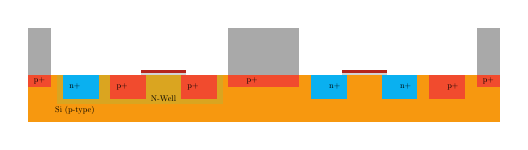
\begin{tikzpicture}[node distance = 3cm, auto, thick,scale=\CrossAndTopSectionBig, every node/.style={transform shape}]
		% substrate
\fill[YellowOrange] (0,0) rectangle (20,2);
\node at (2,0.5) {Si (p-type)};
% n-well
\fill[Goldenrod] (1.25,0.75) rectangle (8.25,2);
\node at (5.75,1) {N-Well};
% body
\fill[ProcessBlue] (1.5,1) rectangle (3,2);
\node at (2,1.5) {n+};
% source
\fill[RedOrange] (3.5,1) rectangle (5,2);
\node at (4,1.5) {p+};
% drain
\fill[RedOrange] (6.5,1) rectangle (8,2);
\node at (7,1.5) {p+};
%% gate:
% gate oxide
\fill[LightGray] (4.8,2) rectangle (6.7,2.1);
% gate poly
\fill[BrickRed] (4.8,2.1) rectangle (6.7,2.2);

%field oxides:
\fill[DarkGray] (0,2) rectangle (1,4);
\fill[DarkGray] (8.5,2) rectangle (11.5,4);
\fill[DarkGray] (19,2) rectangle (20,4);

\fill[RedOrange] (0,1.5) rectangle (1,2);
\fill[RedOrange] (8.5,1.5) rectangle (11.5,2);
\fill[RedOrange] (19,1.5) rectangle (20,2);

\node at (0.5,1.75) {p+};
\node at (9.5,1.75) {p+};
\node at (19.5,1.75) {p+};

%%% nmos:
% body
\fill[RedOrange] (17,1) rectangle (18.5,2);
\node at (18,1.5) {p+};
% source
\fill[ProcessBlue] (15,1) rectangle (16.5,2);
\node at (16,1.5) {n+};
% drain
\fill[ProcessBlue] (12,1) rectangle (13.5,2);
\node at (13,1.5) {n+};

%% gate:
% gate oxide
\fill[LightGray] (13.3,2) rectangle (15.2,2.1);
% gate poly
\fill[BrickRed] (13.3,2.1) rectangle (15.2,2.2);
	\end{tikzpicture}
	\begin{tikzpicture}[node distance = 3cm, auto, thick,scale=\CrossAndTopSectionBig, every node/.style={transform shape}]
		\fill[isolationoxide] (0,0) rectangle (20,10);

% n-well
\fill[nwell] (1,1.25) rectangle (8.5,7.5);

% p-well
\fill[pwell] (11.5,1.25) rectangle (19,7.5);

% gate metal
\fill[gatemetal] (5,0) rectangle (6.5,9);
\fill[gatemetal] (13.5,0) rectangle (15,9);
\fill[gatemetal] (5,8) rectangle (15,10);

% n+
\fill[nimplant] (1.5,2) rectangle (3,6.5);
\fill[nimplant] (12,2) rectangle (13.5,6.5);
\fill[nimplant] (15,2) rectangle (16.5,6.5);

	\end{tikzpicture}
	\caption{N+ implant geometry target}
\end{figure}

The tricky thing here is to have a reasonable implant depth but not too deep because the deeper the junction, the higher the junction capacity which in turn limits the switching performance of the CMOS circuitry.

\begin{figure}[H]
	\centering
	\begin{tikzpicture}[node distance =1cm, auto, thick,scale=\VLSILayout, every node/.style={transform shape}]
		\input{tikz_process_steps/pimplant.layout.tex}
% gate metal
\fill[gatemetal,opacity=\OpacityLayout] (4.8,1.75) rectangle (6.7,8);
\fill[gatemetal,opacity=\OpacityLayout] (13.3,1.75) rectangle (15.2,8);
\fill[gatemetal,opacity=\OpacityLayout] (4.8,8) rectangle (15.2,10);


% n+
\fill[nimplant,opacity=\OpacityLayout] (1.5,2) rectangle (3,6.5);
\fill[nimplant,opacity=\OpacityLayout] (12,2) rectangle (13.5,6.5);
\fill[nimplant,opacity=\OpacityLayout] (15,2) rectangle (16.5,6.5);

	\end{tikzpicture}
	\caption{N+ layout}
	\label{nimplant_layout}
\end{figure}

An example layout of p-implants can be seen in \autoref{nimplant_layout}, the mask is being extracted from the layer "n\_plus\_select".

Also important to notice is that this example layout is just for demonstration purposes only, please have a look at the standard cell documentation for the actual layouts. 

\newpage

\subsection{Patterning}

The resist is being deposited using spin coating and then baked depending on the baking time for the specific resist.
The layout for being exposed onto the resist is being extracted from the "n\_plus\_select" layer within the GDS2 file onto a \textbf{bright field} mask.
The requirement is a \textbf{negative} tone resist.

\begin{figure}[H]
	\centering
	\begin{tikzpicture}[node distance = 3cm, auto, thick,scale=\CrossAndTopSection, every node/.style={transform shape}]
		\input{tikz_process_steps/pwell.a.tex}
\fill[gateoxide] (4.8,2) rectangle (6.7,2.3);
\fill[gateoxide] (13.3,2) rectangle (15.2,2.3);
\fill[gatemetal] (4.8,2.3) rectangle (6.7,2.6);
\fill[gatemetal] (13.3,2.3) rectangle (15.2,2.6);

	\end{tikzpicture}
	\begin{tikzpicture}[node distance = 3cm, auto, thick,scale=\CrossAndTopSection, every node/.style={transform shape}]
		\input{tikz_process_steps/nimplant.patterning.at.tex}
	\end{tikzpicture}
	\drawStepArrow{Mask: nselect}
	\begin{tikzpicture}[node distance = 3cm, auto, thick,scale=\CrossAndTopSection, every node/.style={transform shape}]
		% resist
\fill[resist] (0,2.0) rectangle (1.25,6.0);
\fill[resist] (3,2.0) rectangle (11.75,6.0);
\fill[resist] (17,2.0) rectangle (20,6.0);

\input{tikz_process_steps/nimplant.oxide_growth.b.tex}

	\end{tikzpicture}
	\begin{tikzpicture}[node distance = 3cm, auto, thick,scale=\CrossAndTopSection, every node/.style={transform shape}]
		\fill[resist] (0,0) rectangle (20,12);

% n+
\fill[isolationoxide] (1.5,2) rectangle (3,6.5);
\fill[isolationoxide] (12,2) rectangle (13.5,6.5);
\fill[isolationoxide] (15,2) rectangle (16.5,6.5);
	\end{tikzpicture}
	\caption{N+ region resist mask}
\end{figure}

The thickness of the resist layer and the baking duration will variate depending on the specific equipment for which this process will be implemented with.
Also after the exposure and development, the hard baking shouldn't be forgotten!

\newpage

\subsection{Implantation}\label{nimplant_implant_step}

We now need to bring in the carriers in order to build the n-junctions.

\begin{figure}[H]
	\centering
	\begin{tikzpicture}[node distance = 3cm, auto, thick,scale=\CrossSectionOnly, every node/.style={transform shape}]
		% oxide
\fill[isolationoxide] (0,2) rectangle (1.25,3.5);
\fill[isolationoxide] (3,2) rectangle (11.75,3.5);
\fill[isolationoxide] (17,2) rectangle (20,3.5);

\forloop{ct}{0}{\value{ct} < 21}
{
	\draw [->] (\value{ct},5) -- (\value{ct},4);
	\node at (\value{ct},5.2) {P$^{31}$};
}

\input{tikz_process_steps/pwell.a.tex}
\fill[gateoxide] (4.8,2) rectangle (6.7,2.3);
\fill[gateoxide] (13.3,2) rectangle (15.2,2.3);
\fill[gatemetal] (4.8,2.3) rectangle (6.7,2.6);
\fill[gatemetal] (13.3,2.3) rectangle (15.2,2.6);
	\end{tikzpicture}
	\drawStepArrow{Boron implant}
	\begin{tikzpicture}[node distance = 3cm, auto, thick,scale=\CrossSectionOnly, every node/.style={transform shape}]
		% resist
\fill[resist] (0,2.0) rectangle (0.75,5.0);
\fill[resist] (3.25,2.0) rectangle (11.25,5.0);
\fill[resist] (16.25,2.0) rectangle (20,5.0);

\input{tikz_process_steps/gate.a.tex}

\shade[upper left = nimplant, upper right = nimplant, lower right = nwell, lower left = nwell,] (1.5,1.5) rectangle (2.5,2);
\node at (2,1.65) {n+};
\shade[upper left = nimplant, upper right = nimplant, lower right = pwell, lower left = pwell,] (12.0,1.5) rectangle (13.0,2);
\node at (12.5,1.65) {n+};
\shade[upper left = nimplant, upper right = nimplant, lower right = pwell, lower left = pwell,] (14.5,1.5) rectangle (15.5,2);
\node at (15,1.65) {n+};



	\end{tikzpicture} \\
	\caption{N+ implant process}
\end{figure}

\textbf{Possible approaches}:
\begin{itemize}
	\item \textbf{"CF-3000 Implanter (IMP-3000)" from HKUST} \\
	At HKUST we have an implanter which gives us better control over the initial surface concentration. \\
	These steps are needed to arrive with the desired geometry:
	The nselect is implanted with a Phosphorus ($P^{31}$) dose of $2.5\times10^{12}cm^{-2}$ at an energy of 35 keV (43nm$\pm$18nm deep)
\end{itemize}

\subsection{Resist strip}

Now we need to remove the contaminants for further processing.

\begin{figure}[H]
	\centering
	\begin{tikzpicture}[node distance = 3cm, auto, thick,scale=\CrossSectionOnly, every node/.style={transform shape}]
		% resist
\fill[resist] (0,2.0) rectangle (0.75,5.0);
\fill[resist] (3.25,2.0) rectangle (11.25,5.0);
\fill[resist] (16.25,2.0) rectangle (20,5.0);

\input{tikz_process_steps/nimplant.cleaning.b.tex}


	\end{tikzpicture}
	\drawStepArrow{}
	\begin{tikzpicture}[node distance = 3cm, auto, thick,scale=\CrossSectionOnly, every node/.style={transform shape}]
		\input{tikz_process_steps/pwell.a.tex}
\fill[gateoxide] (4.8,2) rectangle (6.7,2.3);
\fill[gateoxide] (13.3,2) rectangle (15.2,2.3);
\fill[gatemetal] (4.8,2.3) rectangle (6.7,2.6);
\fill[gatemetal] (13.3,2.3) rectangle (15.2,2.6);

\shade[upper left = nimplant, upper right = nimplant, lower right = nwell, lower left = nwell,] (1.5,1.5) rectangle (2.5,2);
\node at (2,1.65) {n+};
\shade[upper left = nimplant, upper right = nimplant, lower right = pwell, lower left = pwell,] (12.0,1.5) rectangle (13.0,2);
\node at (12.5,1.65) {n+};
\shade[upper left = nimplant, upper right = nimplant, lower right = pwell, lower left = pwell,] (14.5,1.5) rectangle (15.5,2);
\node at (15,1.65) {n+};


	\end{tikzpicture}
	\caption{Resist removal}
\end{figure}

We strip the resist, rinse and perform sulfuric cleaning.

\newpage


\newpage
\subsection{p+ Implant}\label{pimplant_chapter}

For the bulk of the NMOS transistors and for the source and drain of the PMOS transistors highly doped  p+ areas are required.

In this step we're going to build these.

\begin{figure}[H]
	\centering
	\begin{tikzpicture}[node distance = 3cm, auto, thick,scale=\CrossAndTopSectionBig, every node/.style={transform shape}]
		% substrate
\fill[YellowOrange] (0,0) rectangle (20,2);
\node at (2,0.5) {Si (p-type)};
% n-well
\fill[Goldenrod] (1.25,0.75) rectangle (8.25,2);
\node at (5.75,1) {N-Well};
% body
\fill[ProcessBlue] (1.5,1) rectangle (3,2);
\node at (2,1.5) {n+};
% source
\fill[RedOrange] (3.5,1) rectangle (5,2);
\node at (4,1.5) {p+};
% drain
\fill[RedOrange] (6.5,1) rectangle (8,2);
\node at (7,1.5) {p+};
%% gate:
% gate oxide
\fill[LightGray] (4.8,2) rectangle (6.7,2.1);
% gate poly
\fill[BrickRed] (4.8,2.1) rectangle (6.7,2.2);

%field oxides:
\fill[DarkGray] (0,2) rectangle (1,4);
\fill[DarkGray] (8.5,2) rectangle (11.5,4);
\fill[DarkGray] (19,2) rectangle (20,4);

\fill[RedOrange] (0,1.5) rectangle (1,2);
\fill[RedOrange] (8.5,1.5) rectangle (11.5,2);
\fill[RedOrange] (19,1.5) rectangle (20,2);

\node at (0.5,1.75) {p+};
\node at (9.5,1.75) {p+};
\node at (19.5,1.75) {p+};

%%% nmos:
% body
\fill[RedOrange] (17,1) rectangle (18.5,2);
\node at (18,1.5) {p+};
% source
\fill[ProcessBlue] (15,1) rectangle (16.5,2);
\node at (16,1.5) {n+};
% drain
\fill[ProcessBlue] (12,1) rectangle (13.5,2);
\node at (13,1.5) {n+};

%% gate:
% gate oxide
\fill[LightGray] (13.3,2) rectangle (15.2,2.1);
% gate poly
\fill[BrickRed] (13.3,2.1) rectangle (15.2,2.2);
\fill[pimplant] (3.5,1) rectangle (5,2);
\node at (4,1.5) {p+};
\fill[pimplant] (6.5,1) rectangle (8,2);
\node at (7,1.5) {p+};
\fill[pimplant] (17,1) rectangle (18.5,2);
\node at (18,1.5) {p+};
	\end{tikzpicture}
	\caption{P+ implant geometry target}
\end{figure}

The tricky thing here is to have a reasonable implant depth but not too deep because the deeper the junction, the higher the junction capacity which in turn limits the switching performance of the CMOS circuitry.

Also important to notice is that the implantation energy must not be too high, otherwise the dopants may leak through the polysilicon gate.

The pselect is implanted with a Boron ($B^{11}$) dose of $2.5\times10^{12}cm^{-2}$ at an energy of 20 keV  (43nm$\pm$18nm deep)


\newpage
\section{Silicification}\label{step_silicification}

Titanium silicide is one of the first SALICIDE material introduced in ULSI devices owing to its low resistivity, high thermal stability, ease in deposition and compatibility with silicon processes.
Titanium has been one of the familiar materials in ULSI productions, which is also an important advantage in practical use of titanium SALICIDE.\footnote{A Study on Formation of High Resistivity Phases of Nickel Silicide at Small Area and its Solution for Scaled CMOS Devices, 07D53437, Ryuji Tomita}

\begin{figure}[H]
	\centering
	\begin{tikzpicture}[node distance = 3cm, auto, thick,scale=\CrossAndTopSectionBig, every node/.style={transform shape}]
		\input{tikz_process_steps/nimplant.a.tex}
\fill[pimplant] (3.5,1) rectangle (5,2);
\node at (4,1.5) {p+};
\fill[pimplant] (6.5,1) rectangle (8,2);
\node at (7,1.5) {p+};
\fill[pimplant] (17,1) rectangle (18.5,2);
\node at (18,1.5) {p+};

\filldraw[line width=0, isolationoxide] (5.75,2.0) -- (5.5,2.0) -- (5.75,3.0);
\filldraw[line width=0, isolationoxide] (6.75,2.0) -- (7.0,2.0) -- (6.75,3.0);

\filldraw[line width=0, isolationoxide] (11.25,2.0) -- (11.0,2.0) -- (11.25,3.0);
\filldraw[line width=0, isolationoxide] (12.5,2.0) -- (12.25,2.0) -- (12.25,3.0);

\filldraw[line width=0, isolationoxide] (22.75,2.4) -- (22.6,2.4) -- (22.75,3.4);
\filldraw[line width=0, isolationoxide] (23.75,2.4) -- (23.9,2.4) -- (23.75,3.4);

\fill[silicide] (1.5,1.9) rectangle (2.5,2);
\fill[silicide] (4.5,1.9) rectangle (5.5,2);
\fill[silicide] (5.75,2.9) rectangle (6.75,3.0);
\fill[silicide] (7,1.9) rectangle (8,2);

\fill[silicide] (10.0,1.9) rectangle (11.0,2);
\fill[silicide] (11.25,2.9) rectangle (12.25,3.0);
\fill[silicide] (12.5,1.9) rectangle (13.5,2);
\fill[silicide] (15.5,1.9) rectangle (16.5,2);

\fill[silicide] (19.0,1.9) rectangle (20.0,2);

\fill[silicide] (22.0,1.9) rectangle (22.6,2.0);
\fill[silicide] (22.75,3.3) rectangle (23.75,3.4);
\fill[silicide] (23.9,1.9) rectangle (24.5,2.0);

\fill[silicide] (27.0,1.9) rectangle (27.75,2.0);
\fill[silicide] (28.5,1.9) rectangle (29.0,2.0);
\fill[silicide] (29.75,1.9) rectangle (30.5,2.0);
\fill[silicide] (31.25,1.9) rectangle (31.75,2.0);
\fill[silicide] (32.5,1.9) rectangle (33.5,2.0);

\fill[silicide] (35.75,1.9) rectangle (36.5,2.0);
\fill[silicide] (37.25,1.9) rectangle (37.75,2.0);
\fill[silicide] (38.5,1.9) rectangle (39.0,2.0);
\fill[silicide] (39.75,1.9) rectangle (40.25,2.0);
\fill[silicide] (41.0,1.9) rectangle (41.75,2.0);

% diode contacts
\fill[silicide] (43.0,3.4) rectangle (44.0,3.5);
\fill[silicide] (47.0,3.4) rectangle (48.0,3.5);

% resistor contacts
\fill[silicide] (49.0,3.4) rectangle (49.5,3.5);
\fill[silicide] (53.5,3.4) rectangle (54.0,3.5);

	\end{tikzpicture}
	\caption{Silicide geometry target}
	\label{policide_silicide_sections}
\end{figure}

In order to reduce the gate contact resistance as well as the source and drain resistance and in order to provide a more effective etch stop when plasma etching the contact windows to drain, source and gate, silicide/polycide is being added to the wafer as shown in \autoref{policide_silicide_sections}.

The side walls\footnote{\url{http://www.fujitsu.com/jp/group/mifs/en/resources/news/library/tech-intro/process/side-wall.html}} are required in order avoid short circuits between the junction and the gate.

When titanium and silicon are brought into contact and heated at temperatures above 800 \degree C (in the presence of excess silicon) $Ti Si_2$ forms.

The $TiSi_2$ has a resistivity of $12-20 \mu\Omega - cm$.

The basic formation process of titanium SALICIDE is as follows:

A thin titanium film of roughly 30 nm thickness is deposited on an entire wafer with MOSFETs structure.

The deposited Ti film reacts with the exposed silicon areas such as the source/drain area and polysilicon gate electrodes during the annealing at 800\degree C in Argon atmosphere.

Then, the unreacted titanium film on the dielectric layer such as $SiO_2$ or SiN is selectively etched by APM (Ammonia and Hydrogen Peroxide Mixture) solution for around 2-3 minutes.

\newpage

\subsection{Nitride deposition}\label{nitride_spacers_deposition}

The thickness of this CVD deposited nitride layer will be the width of the spacer after having used highly anisotropic etching in the next few steps, for this reason the thickness of the nitride decides over the distance between the silicide and the gate oxide.

Considering, due to the edge effects during dry etching, the thickness of the nitride has to be less than 25\% of the polysilicon thickness, we choose 50nm for the nitride thickness.

\begin{figure}[H]
	\centering
	\begin{tikzpicture}[node distance = 3cm, auto, thick,scale=\CrossSectionOnly, every node/.style={transform shape}]
		\input{tikz_process_steps/nimplant.a.tex}
\fill[pimplant] (3.5,1) rectangle (5,2);
\node at (4,1.5) {p+};
\fill[pimplant] (6.5,1) rectangle (8,2);
\node at (7,1.5) {p+};
\fill[pimplant] (17,1) rectangle (18.5,2);
\node at (18,1.5) {p+};
	\end{tikzpicture}
	\drawStepArrow{Silicon oxide deposition}
	\begin{tikzpicture}[node distance = 3cm, auto, thick,scale=\CrossSectionOnly, every node/.style={transform shape}]
		\fill[isolationoxide] (0,2.0) rectangle (20,3.5);
\input{tikz_process_steps/nimplant.a.tex}
\fill[pimplant] (3.5,1) rectangle (5,2);
\node at (4,1.5) {p+};
\fill[pimplant] (6.5,1) rectangle (8,2);
\node at (7,1.5) {p+};
\fill[pimplant] (17,1) rectangle (18.5,2);
\node at (18,1.5) {p+};

	\end{tikzpicture}
	\caption{Oxide layer}
\end{figure}

The deposition rates might variate between LPCVDs and recipes. It's at the discretion of the operation engineer to achieve those 50nm.

\newpage

\subsection{Spacer etching}

Now we have to etch our nitride as anisotropic as possible.

This means that the etching mostly only comes "from above" with a few to nearly none horizontal etching.

Thit means the etching process only "sees" the sidewall as a "thicker layer" and starts etching downward.

\begin{figure}[H]
	\centering
	\begin{tikzpicture}[node distance = 3cm, auto, thick,scale=\CrossSectionOnly, every node/.style={transform shape}]
		\coveringlayer{nitride}{0.5}{0.5}

\filldraw[line width=0, nitride] ( 4.50,\STIIslandSurface) rectangle ( 6.50,\STIIslandSurface+1.9);
\filldraw[line width=0, nitride] (11.50,\STIIslandSurface) rectangle (13.50,\STIIslandSurface+1.9);
\filldraw[line width=0, nitride] (21.40,\STIIslandSurface) rectangle (23.40,\STIIslandSurface+2.1);

\fill[nitride] (42.50,\STIIslandSurface+0.75) rectangle (48.50,\polytop+1.25);
\fill[nitride] (44.5,\polytop+0.75) rectangle (46.5,\implantstoptop+0.5);

\fill[nitride] (48.00,\STIIslandSurface+0.75) rectangle (55.00,\polytop+1.25);

\input{tikz_process_steps/pimplant.a.tex}


	\end{tikzpicture}
	\drawStepArrow{Sputter etching}
	\begin{tikzpicture}[node distance = 3cm, auto, thick,scale=\CrossSectionOnly, every node/.style={transform shape}]
		\filldraw[line width=0, nitride] (5.00,\STIIslandSurface) -- (4.50,\STIIslandSurface) -- (5.00,\STIIslandSurface+1.4);
\filldraw[line width=0, nitride] (6.00,\STIIslandSurface) -- (6.50,\STIIslandSurface) -- (6.00,\STIIslandSurface+1.4);

\filldraw[line width=0, nitride] (12.00,\STIIslandSurface) -- (11.50,\STIIslandSurface) -- (12.00,\STIIslandSurface+1.4);
\filldraw[line width=0, nitride] (13.50,\STIIslandSurface) -- (13.00,\STIIslandSurface) -- (13.00,\STIIslandSurface+1.4);

\filldraw[line width=0, nitride] (21.40,\STIIslandSurface) -- (21.90,\STIIslandSurface) -- (21.90,\STIIslandSurface+1.6);
\filldraw[line width=0, nitride] (22.90,\STIIslandSurface) -- (23.40,\STIIslandSurface) -- (22.90,\STIIslandSurface+1.6);

\fill[nitride] (44.0,\polytop+0.75) rectangle (44.8,\polytop+1.25);
\fill[nitride] (44.5,\polytop+0.75) rectangle (46.5,\implantstoptop+0.5);
\fill[nitride] (46.2,\polytop+0.75) rectangle (47.0,\polytop+1.25);

\fill[nitride] (49.5,\polytop+0.75) rectangle (53.5,\polytop+1.25);

\input{tikz_process_steps/nimplant.a.tex}
\fill[pimplant] (3.5,1) rectangle (5,2);
\node at (4,1.5) {p+};
\fill[pimplant] (6.5,1) rectangle (8,2);
\node at (7,1.5) {p+};
\fill[pimplant] (17,1) rectangle (18.5,2);
\node at (18,1.5) {p+};


	\end{tikzpicture}
	\caption{Anisotropic etching}
\end{figure}

After that we will have our desired spacer geometry forming as well as any potentially resist covered area (if silicide block is being used) with sharp etches.

\subsection{Titanium deposition}

We deposit a layer of titanium with a thickness of around 30nm which will then be reacted into titanium-silicide and titanium-polycide respectively in the further steps.

\begin{figure}[H]
	\centering
	\begin{tikzpicture}[node distance = 3cm, auto, thick,scale=\CrossSectionOnly, every node/.style={transform shape}]
		\filldraw[line width=0, nitride] (5.00,\STIIslandSurface) -- (4.50,\STIIslandSurface) -- (5.00,\STIIslandSurface+1.4);
\filldraw[line width=0, nitride] (6.00,\STIIslandSurface) -- (6.50,\STIIslandSurface) -- (6.00,\STIIslandSurface+1.4);

\filldraw[line width=0, nitride] (12.00,\STIIslandSurface) -- (11.50,\STIIslandSurface) -- (12.00,\STIIslandSurface+1.4);
\filldraw[line width=0, nitride] (13.50,\STIIslandSurface) -- (13.00,\STIIslandSurface) -- (13.00,\STIIslandSurface+1.4);

\filldraw[line width=0, nitride] (21.40,\STIIslandSurface) -- (21.90,\STIIslandSurface) -- (21.90,\STIIslandSurface+1.6);
\filldraw[line width=0, nitride] (22.90,\STIIslandSurface) -- (23.40,\STIIslandSurface) -- (22.90,\STIIslandSurface+1.6);

\fill[nitride] (44.0,\polytop+0.75) rectangle (44.8,\polytop+1.25);
\fill[nitride] (44.5,\polytop+0.75) rectangle (46.5,\implantstoptop+0.5);
\fill[nitride] (46.2,\polytop+0.75) rectangle (47.0,\polytop+1.25);

\fill[nitride] (49.5,\polytop+0.75) rectangle (53.5,\polytop+1.25);

\input{tikz_process_steps/pimplant.a.tex}



	\end{tikzpicture}
	\drawStepArrow{}
	\begin{tikzpicture}[node distance = 3cm, auto, thick,scale=\CrossSectionOnly, every node/.style={transform shape}]
		\coveringlayer{titanium}{0.5}{0.5}

\filldraw[line width=0, titanium] (4.50,\STIIslandSurface+0.5) -- (4.00,\STIIslandSurface+0.5) -- (4.50,\STIIslandSurface+1.9);
\filldraw[line width=0, titanium] (6.50,\STIIslandSurface+0.5) -- (7.00,\STIIslandSurface+0.5) -- (6.50,\STIIslandSurface+1.9);

\filldraw[line width=0, titanium] (11.50,\STIIslandSurface+0.5) -- (11.00,\STIIslandSurface+0.5) -- (11.50,\STIIslandSurface+1.9);
\filldraw[line width=0, titanium] (14.00,\STIIslandSurface+0.5) -- (13.50,\STIIslandSurface+0.5) -- (13.50,\STIIslandSurface+1.9);

\filldraw[line width=0, titanium] (20.90,\STIIslandSurface+0.5) -- (21.40,\STIIslandSurface+0.5) -- (21.40,\STIIslandSurface+2.1);
\filldraw[line width=0, titanium] (23.40,\STIIslandSurface+0.5) -- (23.90,\STIIslandSurface+0.5) -- (23.40,\STIIslandSurface+2.1);

\filldraw[line width=0, titanium] ( 4.50,\STIIslandSurface) rectangle ( 6.50,\STIIslandSurface+1.9);
\filldraw[line width=0, titanium] (11.50,\STIIslandSurface) rectangle (13.50,\STIIslandSurface+1.9);
\filldraw[line width=0, titanium] (21.40,\STIIslandSurface) rectangle (23.40,\STIIslandSurface+2.1);

\fill[titanium] (42.50,\STIIslandSurface+0.75) rectangle (48.50,\polytop+1.25);
\fill[titanium] (43.50,\STIIslandSurface+0.75) rectangle (47.50,\polytop+1.75);
\fill[titanium] (44.00,\STIIslandSurface+0.75) rectangle (47.00,\polytop+2.75);

\fill[titanium] (48.00,\STIIslandSurface+0.75) rectangle (55.00,\polytop+1.25);


\fill[titanium] (49.00,\polytop+0.75) rectangle (54.0,\polytop+1.75);


\filldraw[line width=0, nitride] (5.00,\STIIslandSurface) -- (4.50,\STIIslandSurface) -- (5.00,\STIIslandSurface+1.4);
\filldraw[line width=0, nitride] (6.00,\STIIslandSurface) -- (6.50,\STIIslandSurface) -- (6.00,\STIIslandSurface+1.4);

\filldraw[line width=0, nitride] (12.00,\STIIslandSurface) -- (11.50,\STIIslandSurface) -- (12.00,\STIIslandSurface+1.4);
\filldraw[line width=0, nitride] (13.50,\STIIslandSurface) -- (13.00,\STIIslandSurface) -- (13.00,\STIIslandSurface+1.4);

\filldraw[line width=0, nitride] (21.40,\STIIslandSurface) -- (21.90,\STIIslandSurface) -- (21.90,\STIIslandSurface+1.6);
\filldraw[line width=0, nitride] (22.90,\STIIslandSurface) -- (23.40,\STIIslandSurface) -- (22.90,\STIIslandSurface+1.6);

\fill[nitride] (44.0,\polytop+0.75) rectangle (44.8,\polytop+1.25);
\fill[nitride] (44.5,\polytop+0.75) rectangle (46.5,\implantstoptop+0.5);
\fill[nitride] (46.2,\polytop+0.75) rectangle (47.0,\polytop+1.25);

\fill[nitride] (49.5,\polytop+0.75) rectangle (53.5,\polytop+1.25);

\input{tikz_process_steps/pimplant.a.tex}



	\end{tikzpicture}
	\caption{Titanium deposition}
\end{figure}

The titanium can either be applied by sputtering or by chemical deposition.

\newpage

\subsection{Silicide formation}

The deposited Ti film reacts with the exposed silicon areas such as the source/drain area and polysilicon gate electrodes during RTP (Rapid Thermal Processing) at 800\degreesC in Argon ambient for 30 seconds.

In this annealing step the $Ti Si_2$ is formed.

\begin{figure}[H]
	\centering
	\begin{tikzpicture}[node distance = 3cm, auto, thick,scale=\CrossSectionOnly, every node/.style={transform shape}]
		\coveringlayer{titanium}{0.5}{0.5}

\filldraw[line width=0, titanium] (4.50,\STIIslandSurface+0.5) -- (4.00,\STIIslandSurface+0.5) -- (4.50,\STIIslandSurface+1.9);
\filldraw[line width=0, titanium] (6.50,\STIIslandSurface+0.5) -- (7.00,\STIIslandSurface+0.5) -- (6.50,\STIIslandSurface+1.9);

\filldraw[line width=0, titanium] (11.50,\STIIslandSurface+0.5) -- (11.00,\STIIslandSurface+0.5) -- (11.50,\STIIslandSurface+1.9);
\filldraw[line width=0, titanium] (14.00,\STIIslandSurface+0.5) -- (13.50,\STIIslandSurface+0.5) -- (13.50,\STIIslandSurface+1.9);

\filldraw[line width=0, titanium] (20.90,\STIIslandSurface+0.5) -- (21.40,\STIIslandSurface+0.5) -- (21.40,\STIIslandSurface+2.1);
\filldraw[line width=0, titanium] (23.40,\STIIslandSurface+0.5) -- (23.90,\STIIslandSurface+0.5) -- (23.40,\STIIslandSurface+2.1);

\filldraw[line width=0, titanium] ( 4.50,\STIIslandSurface) rectangle ( 6.50,\STIIslandSurface+1.9);
\filldraw[line width=0, titanium] (11.50,\STIIslandSurface) rectangle (13.50,\STIIslandSurface+1.9);
\filldraw[line width=0, titanium] (21.40,\STIIslandSurface) rectangle (23.40,\STIIslandSurface+2.1);

\fill[titanium] (42.50,\STIIslandSurface+0.75) rectangle (48.50,\polytop+1.25);
\fill[titanium] (43.50,\STIIslandSurface+0.75) rectangle (47.50,\polytop+1.75);
\fill[titanium] (44.00,\STIIslandSurface+0.75) rectangle (47.00,\polytop+2.75);

\fill[titanium] (48.00,\STIIslandSurface+0.75) rectangle (55.00,\polytop+1.25);


\fill[titanium] (49.00,\polytop+0.75) rectangle (54.0,\polytop+1.75);


\input{tikz_process_steps/silicification.sputter_etching.b.tex}


	\end{tikzpicture}
	\drawStepArrow{}
	\begin{tikzpicture}[node distance = 3cm, auto, thick,scale=\CrossSectionOnly, every node/.style={transform shape}]
		\fill[titanium] (0,2.0) rectangle (20,2.5);
\fill[titanium] (4.5,2.0) rectangle (7,3.5);
\fill[titanium] (13,2.0) rectangle (15.5,3.5);
\filldraw[line width=0, titanium] (4.5,2.5) -- (4.0,2.5) -- (4.5,3.5);
\filldraw[line width=0, titanium] (7.0,2.5) -- (7.5,2.5) -- (7.0,3.5);
\filldraw[line width=0, titanium] (13.0,2.5) -- (12.5,2.5) -- (13.0,3.5);
\filldraw[line width=0, titanium] (15.5,2.5) -- (16.0,2.5) -- (15.5,3.5);

\filldraw[line width=0, isolationoxide] (5,2.0) -- (4.5,2.0) -- (5,3.0);
\filldraw[line width=0, isolationoxide] (6.5,2.0) -- (7.0,2.0) -- (6.5,3.0);
\filldraw[line width=0, isolationoxide] (13.5,2.0) -- (13.0,2.0) -- (13.5,3.0);
\filldraw[line width=0, isolationoxide] (15,2.0) -- (15.5,2.0) -- (15,3.0);

\input{tikz_process_steps/pimplant.a.tex}

\fill[silicide] (1.25,1.8) rectangle (4.5,2);
\fill[silicide] (5,2.8) rectangle (6.5,3.0);
\fill[silicide] (7,1.8) rectangle (8.25,2);

\fill[silicide] (11.75,1.8) rectangle (13,2);
\fill[silicide] (13.5,2.8) rectangle (15,3.0);
\fill[silicide] (15.5,1.8) rectangle (18.75,2);
	\end{tikzpicture}
	\caption{Reaction 1}
\end{figure}

The resulting $Ti Si_2$ film will be around 77nm in tickness with around 20nm unreacted titanium left on top.

A color change can be observed of the titanium on top of the oxide.

\subsection{Metal removal}

The unreacted titanium film on the dielectric layer such as $SiO_2$ or $SiN$ is selectively etched by APM (Ammonia and Hydrogen Peroxide Mixture) solution.

\begin{figure}[H]
	\centering
	\begin{tikzpicture}[node distance = 3cm, auto, thick,scale=\CrossSectionOnly, every node/.style={transform shape}]
		\fill[titanium] (0,2.0) rectangle (20,2.5);
\fill[titanium] (4.5,2.0) rectangle (7,3.5);
\fill[titanium] (13,2.0) rectangle (15.5,3.5);
\filldraw[line width=0, titanium] (4.5,2.5) -- (4.0,2.5) -- (4.5,3.5);
\filldraw[line width=0, titanium] (7.0,2.5) -- (7.5,2.5) -- (7.0,3.5);
\filldraw[line width=0, titanium] (13.0,2.5) -- (12.5,2.5) -- (13.0,3.5);
\filldraw[line width=0, titanium] (15.5,2.5) -- (16.0,2.5) -- (15.5,3.5);

\input{tikz_process_steps/silicification.rtp2.b.tex}

	\end{tikzpicture}
	\drawStepArrow{}
	\begin{tikzpicture}[node distance = 3cm, auto, thick,scale=\CrossSectionOnly, every node/.style={transform shape}]
		\filldraw[line width=0, nitride] (5.00,\STIIslandSurface) -- (4.50,\STIIslandSurface) -- (5.00,\STIIslandSurface+1.4);
\filldraw[line width=0, nitride] (6.00,\STIIslandSurface) -- (6.50,\STIIslandSurface) -- (6.00,\STIIslandSurface+1.4);

\filldraw[line width=0, nitride] (12.00,\STIIslandSurface) -- (11.50,\STIIslandSurface) -- (12.00,\STIIslandSurface+1.4);
\filldraw[line width=0, nitride] (13.50,\STIIslandSurface) -- (13.00,\STIIslandSurface) -- (13.00,\STIIslandSurface+1.4);

\filldraw[line width=0, nitride] (21.40,\STIIslandSurface) -- (21.90,\STIIslandSurface) -- (21.90,\STIIslandSurface+1.6);
\filldraw[line width=0, nitride] (22.90,\STIIslandSurface) -- (23.40,\STIIslandSurface) -- (22.90,\STIIslandSurface+1.6);

\fill[nitride] (44.0,\polytop+0.75) rectangle (44.8,\polytop+1.25);
\fill[nitride] (44.5,\polytop+0.75) rectangle (46.5,\implantstoptop+0.5);
\fill[nitride] (46.2,\polytop+0.75) rectangle (47.0,\polytop+1.25);

\fill[nitride] (49.5,\polytop+0.75) rectangle (53.5,\polytop+1.25);

\input{tikz_process_steps/nimplant.a.tex}
\fill[pimplant] (3.5,1) rectangle (5,2);
\node at (4,1.5) {p+};
\fill[pimplant] (6.5,1) rectangle (8,2);
\node at (7,1.5) {p+};
\fill[pimplant] (17,1) rectangle (18.5,2);
\node at (18,1.5) {p+};

\fill[silicide] ( 1.35,\STIIslandSurface-0.1) rectangle ( 2.35,\STIIslandSurface);
\fill[silicide] ( 2.70,\STIIslandSurface-0.1) rectangle ( 4.50,\STIIslandSurface);
\fill[silicide] ( 5.00,\STIIslandSurface+1.3) rectangle ( 6.00,\STIIslandSurface+1.4);
\fill[silicide] ( 6.50,\STIIslandSurface-0.1) rectangle ( 8.15,\STIIslandSurface);

\fill[silicide] ( 9.85,\STIIslandSurface-0.1) rectangle (11.50,\STIIslandSurface);
\fill[silicide] (12.00,\STIIslandSurface+1.3) rectangle (13.00,\STIIslandSurface+1.4);
\fill[silicide] (13.50,\STIIslandSurface-0.1) rectangle (15.25,\STIIslandSurface);
\fill[silicide] (15.60,\STIIslandSurface-0.1) rectangle (16.60,\STIIslandSurface);

\fill[silicide] (19.20,\STIIslandSurface-0.1) rectangle (20.20,\STIIslandSurface);
\fill[silicide] (20.60,\STIIslandSurface-0.1) rectangle (21.40,\STIIslandSurface);
\fill[silicide] (21.90,\STIIslandSurface+1.5) rectangle (22.90,\STIIslandSurface+1.6);
\fill[silicide] (23.40,\STIIslandSurface-0.1) rectangle (24.20,\STIIslandSurface);

\fill[silicide] (26.90,\STIIslandSurface-0.1) rectangle (27.90,\STIIslandSurface);
\fill[silicide] (28.35,\STIIslandSurface-0.1) rectangle (29.35,\STIIslandSurface);
\fill[silicide] (29.80,\STIIslandSurface-0.1) rectangle (30.80,\STIIslandSurface);
\fill[silicide] (31.25,\STIIslandSurface-0.1) rectangle (32.15,\STIIslandSurface);
\fill[silicide] (32.60,\STIIslandSurface-0.1) rectangle (33.60,\STIIslandSurface);

\fill[silicide] (35.60,\STIIslandSurface-0.1) rectangle (36.50,\STIIslandSurface);
\fill[silicide] (36.95,\STIIslandSurface-0.1) rectangle (37.85,\STIIslandSurface);
\fill[silicide] (38.30,\STIIslandSurface-0.1) rectangle (39.20,\STIIslandSurface);
\fill[silicide] (39.65,\STIIslandSurface-0.1) rectangle (40.55,\STIIslandSurface);
\fill[silicide] (41.00,\STIIslandSurface-0.1) rectangle (41.90,\STIIslandSurface);

% diode contacts
\fill[silicide] (43.00,\STIIslandSurface+2.0) rectangle (44.00,\STIIslandSurface+2.15);
\fill[silicide] (47.00,\STIIslandSurface+2.0) rectangle (48.00,\STIIslandSurface+2.15);

	\end{tikzpicture}
	\caption{Titanium etch}
\end{figure}

After 2-3 minutes in APM, at room temperature, with a bit mechanical help, all the unreacted Titanium should be gone and the oxide should become visible again.

\newpage
\subsection{Contacts}\label{chapter_contact}

Now we have to build the first set of vias connecting the first metal layer to the active area.
These vias are in the fringe between front-end and back-end process.

\begin{figure}[H]
	\centering
	\begin{tikzpicture}[node distance = 3cm, auto, thick,scale=\CrossAndTopSectionBig, every node/.style={transform shape}]
		\fill[isolationoxide] (0,0) rectangle (55.0,\LowerMetal);

\paintcontacts{white}{white}{white}

\input{tikz_process_steps/pimplant.a.tex}

\filldraw[line width=0, isolationoxide] (5.75,2.0) -- (5.5,2.0) -- (5.75,3.0);
\filldraw[line width=0, isolationoxide] (6.75,2.0) -- (7.0,2.0) -- (6.75,3.0);

\filldraw[line width=0, isolationoxide] (11.25,2.0) -- (11.0,2.0) -- (11.25,3.0);
\filldraw[line width=0, isolationoxide] (12.5,2.0) -- (12.25,2.0) -- (12.25,3.0);

\filldraw[line width=0, isolationoxide] (22.75,2.4) -- (22.6,2.4) -- (22.75,3.4);
\filldraw[line width=0, isolationoxide] (23.75,2.4) -- (23.9,2.4) -- (23.75,3.4);

\fill[silicide] (1.5,1.9) rectangle (2.5,2);
\fill[silicide] (4.5,1.9) rectangle (5.5,2);
\fill[silicide] (5.75,2.9) rectangle (6.75,3.0);
\fill[silicide] (7,1.9) rectangle (8,2);

\fill[silicide] (10.0,1.9) rectangle (11.0,2);
\fill[silicide] (11.25,2.9) rectangle (12.25,3.0);
\fill[silicide] (12.5,1.9) rectangle (13.5,2);
\fill[silicide] (15.5,1.9) rectangle (16.5,2);

\fill[silicide] (19.0,1.9) rectangle (20.0,2);

\fill[silicide] (22.0,1.9) rectangle (22.6,2.0);
\fill[silicide] (22.75,3.3) rectangle (23.75,3.4);
\fill[silicide] (23.9,1.9) rectangle (24.5,2.0);

\fill[silicide] (27.0,1.9) rectangle (27.75,2.0);
\fill[silicide] (28.5,1.9) rectangle (29.0,2.0);
\fill[silicide] (29.75,1.9) rectangle (30.5,2.0);
\fill[silicide] (31.25,1.9) rectangle (31.75,2.0);
\fill[silicide] (32.5,1.9) rectangle (33.5,2.0);

\fill[silicide] (35.75,1.9) rectangle (36.5,2.0);
\fill[silicide] (37.25,1.9) rectangle (37.75,2.0);
\fill[silicide] (38.5,1.9) rectangle (39.0,2.0);
\fill[silicide] (39.75,1.9) rectangle (40.25,2.0);
\fill[silicide] (41.0,1.9) rectangle (41.75,2.0);

% diode contacts
\fill[silicide] (43.0,3.4) rectangle (44.0,3.5);
\fill[silicide] (47.0,3.4) rectangle (48.0,3.5);

% resistor contacts
\fill[silicide] (49.0,3.4) rectangle (49.5,3.5);
\fill[silicide] (53.5,3.4) rectangle (54.0,3.5);


	\end{tikzpicture}
	\caption{Contact geometry target}
	\label{contact_cross_subsections}
\end{figure}

As can be seen in \autoref{contact_cross_subsections}, the goal of this step is purely to deposit a layer of isolation oxide, get the holes into it, down to the silicide and polyside in order to form wires later on.
We do not wanna etch down anywhere else than the silicide/polycide areas because these function as etch stoppers, while everywhere else we might etch further than desired with small variations in etching time which might result in a drastic variation in sheet resistance of the junctions and gate.
In later iterations of this process we might be switching to Tungsten as the metal material for this step.

\newpage
\section{First metal layer}\label{metal}

Now we've got to build the first interconnect wires, connecting the contact vias to the "metal1" wires, which will provide a way to contact to them with the via1 contact layout.

\begin{figure}[H]
	\centering
	\begin{tikzpicture}[node distance = 3cm, auto, thick,scale=\CrossAndTopSectionBig, every node/.style={transform shape}]
		\fill[isolationoxide] (0.0,2.0) rectangle (55.0,\LowerMetal);

\paintcontacts{blue}{brown}{blue}

\input{tikz_process_steps/pimplant.a.tex}

\filldraw[line width=0, isolationoxide] (5.75,2.0) -- (5.5,2.0) -- (5.75,3.0);
\filldraw[line width=0, isolationoxide] (6.75,2.0) -- (7.0,2.0) -- (6.75,3.0);

\filldraw[line width=0, isolationoxide] (11.25,2.0) -- (11.0,2.0) -- (11.25,3.0);
\filldraw[line width=0, isolationoxide] (12.5,2.0) -- (12.25,2.0) -- (12.25,3.0);

\filldraw[line width=0, isolationoxide] (22.75,2.4) -- (22.6,2.4) -- (22.75,3.4);
\filldraw[line width=0, isolationoxide] (23.75,2.4) -- (23.9,2.4) -- (23.75,3.4);

\fill[silicide] (1.5,1.9) rectangle (2.5,2);
\fill[silicide] (4.5,1.9) rectangle (5.5,2);
\fill[silicide] (5.75,2.9) rectangle (6.75,3.0);
\fill[silicide] (7,1.9) rectangle (8,2);

\fill[silicide] (10.0,1.9) rectangle (11.0,2);
\fill[silicide] (11.25,2.9) rectangle (12.25,3.0);
\fill[silicide] (12.5,1.9) rectangle (13.5,2);
\fill[silicide] (15.5,1.9) rectangle (16.5,2);

\fill[silicide] (19.0,1.9) rectangle (20.0,2);

\fill[silicide] (22.0,1.9) rectangle (22.6,2.0);
\fill[silicide] (22.75,3.3) rectangle (23.75,3.4);
\fill[silicide] (23.9,1.9) rectangle (24.5,2.0);

\fill[silicide] (27.0,1.9) rectangle (27.75,2.0);
\fill[silicide] (28.5,1.9) rectangle (29.0,2.0);
\fill[silicide] (29.75,1.9) rectangle (30.5,2.0);
\fill[silicide] (31.25,1.9) rectangle (31.75,2.0);
\fill[silicide] (32.5,1.9) rectangle (33.5,2.0);

\fill[silicide] (35.75,1.9) rectangle (36.5,2.0);
\fill[silicide] (37.25,1.9) rectangle (37.75,2.0);
\fill[silicide] (38.5,1.9) rectangle (39.0,2.0);
\fill[silicide] (39.75,1.9) rectangle (40.25,2.0);
\fill[silicide] (41.0,1.9) rectangle (41.75,2.0);

% diode contacts
\fill[silicide] (43.0,3.4) rectangle (44.0,3.5);
\fill[silicide] (47.0,3.4) rectangle (48.0,3.5);

% resistor contacts
\fill[silicide] (49.0,3.4) rectangle (49.5,3.5);
\fill[silicide] (53.5,3.4) rectangle (54.0,3.5);


	\end{tikzpicture}
	\begin{tikzpicture}[node distance = 3cm, auto, thick,scale=\CrossAndTopSectionBig, every node/.style={transform shape}]
		\fill[isolationoxide] (0,0) rectangle (20,12);
\fill[metal1] (7,8) rectangle (13,12);
\fill[metal1] (1.0,0) rectangle (5.0,12);
\fill[metal1] (6.5,1) rectangle (13.5,7);
\fill[metal1] (8,0) rectangle (12,1);
\fill[metal1] (15.0,0) rectangle (19.0,12);
	\end{tikzpicture}
	\caption{Metal geometry target}
	\label{metal_target}
\end{figure}

As can be seen in \autoref{metal_target}, the goal of this step is purely to etch the wire structure for the first metal layer into the in \autoref{metal_deposition} deposited metal layer, and form wires by doing so.

\begin{figure}[H]
	\centering
	\begin{tikzpicture}[node distance =1cm, auto, thick,scale=\VLSILayout, every node/.style={transform shape}]
		\input{tikz_process_steps/silicification.layout.tex}
%vias

\fill[contact,opacity=\OpacityLayout] (7,1.5) rectangle (8,2.5);
\fill[contact,opacity=\OpacityLayout] (7,3.5) rectangle (8,4.5);
\fill[contact,opacity=\OpacityLayout] (7,5.5) rectangle (8,6.5);

\fill[contact,opacity=\OpacityLayout] (12,1.5) rectangle (13,2.5);
\fill[contact,opacity=\OpacityLayout] (12,3.5) rectangle (13,4.5);
\fill[contact,opacity=\OpacityLayout] (12,5.5) rectangle (13,6.5);

\fill[contact,opacity=\OpacityLayout] (1.5,1.5) rectangle (2.5,2.5);
\fill[contact,opacity=\OpacityLayout] (1.5,3.5) rectangle (2.5,4.5);
\fill[contact,opacity=\OpacityLayout] (1.5,5.5) rectangle (2.5,6.5);

\fill[contact,opacity=\OpacityLayout] (3.5,1.5) rectangle (4.5,2.5);
\fill[contact,opacity=\OpacityLayout] (3.5,3.5) rectangle (4.5,4.5);
\fill[contact,opacity=\OpacityLayout] (3.5,5.5) rectangle (4.5,6.5);

\fill[contact,opacity=\OpacityLayout] (15.5,1.5) rectangle (16.5,2.5);
\fill[contact,opacity=\OpacityLayout] (15.5,3.5) rectangle (16.5,4.5);
\fill[contact,opacity=\OpacityLayout] (15.5,5.5) rectangle (16.5,6.5);

\fill[contact,opacity=\OpacityLayout] (17.5,1.5) rectangle (18.5,2.5);
\fill[contact,opacity=\OpacityLayout] (17.5,3.5) rectangle (18.5,4.5);
\fill[contact,opacity=\OpacityLayout] (17.5,5.5) rectangle (18.5,6.5);

\fill[contact,opacity=\OpacityLayout] (5.5,8.5) rectangle (6.5,9.5); % contact out
\fill[contact,opacity=\OpacityLayout] (7.5,8.5) rectangle (8.5,9.5); % contact out
\fill[contact,opacity=\OpacityLayout] (9.5,8.5) rectangle (10.5,9.5); % contact out
\fill[contact,opacity=\OpacityLayout] (11.5,8.5) rectangle (12.5,9.5); % contact out
\fill[contact,opacity=\OpacityLayout] (13.5,8.5) rectangle (14.5,9.5); % contact out

\draw[|<->|] (7.5,8.25) -- (8.5,8.25);
\node at (8,7.75) {$\lambda$};

\draw[|<->|] (7.25,8.5) -- (7.25,9.5);
\node[rotate=90] at (6.75,8.75) {$\lambda$};

\fill[metal1,opacity=\OpacityLayout] (7,8) rectangle (13,12);
\fill[metal1,opacity=\OpacityLayout] (1.0,0) rectangle (5.0,12);
\fill[metal1,opacity=\OpacityLayout] (6.5,1) rectangle (13.5,7);
\fill[metal1,opacity=\OpacityLayout] (8,0) rectangle (12,1);
\fill[metal1,opacity=\OpacityLayout] (15.0,0) rectangle (19.0,12);

\node at (16,11.5) {VDD};
\node at (2.5,11.5) {GND};
\node at (10,11.5) {Input};
\node at (10,0.5) {Output};
	\end{tikzpicture}
	\caption{First metal layout}
	\label{metal_layout}
\end{figure}

It should be noted again that the via placement and dimensions in \autoref{metal_layout} are solely for demonstration purposes for the process and are in no way the actual standard cell design for the final standard cell lib. \\

In later iterations of this process we might be switching to Tungsten as the metal material for this step so the etching method might change in further releases.

\newpage

\subsection{Metal deposition}\label{metal_deposition}

Now we somehow have got to get the metal onto our silicon oxide in a fashion so that it fills the holes we've etched in \autoref{contact_holes_etch} and touches down onto the silicide/polycide, thus making a contact to the active area.

\begin{figure}[H]
	\centering
	\begin{tikzpicture}[node distance = 3cm, auto, thick,scale=\CrossSectionOnly, every node/.style={transform shape}]
		\input{tikz_process_steps/metal.metal_deposition.a.tex}
	\end{tikzpicture}
	\drawStepArrow{}
	\begin{tikzpicture}[node distance = 3cm, auto, thick,scale=\CrossSectionOnly, every node/.style={transform shape}]
		\input{tikz_process_steps/metal.metal_deposition.b.tex}
	\end{tikzpicture}
	\caption{Metal deposition}
\end{figure}

In order to reach the target of filling the holes in the oxide and having at least another depth worth of space in order to have an enough low resistance of the wire interconnect.
We end up with a target thickness of 4\um.

\textbf{Possible approaches}:
\begin{itemize}
	\item \textbf{"Varian 3180 Sputter (SPT-3180)" from HKUST} \\
	The deposition speed is 16nm/s which gives us a required deposition time of 250 seconds for 4\um.
	\item \textbf{Add your solution here!}
\end{itemize}

\subsection{Pattering}
The resist is being deposited using spin coating and then baked depending on the baking time for the specific resist.
The layout for being exposed onto the resist is being extracted from the "metal1" layer within the GDS2 file onto a \textbf{bright field} mask.
The requirement is a \textbf{positive} tone resist.

\begin{figure}[H]
	\centering
	\begin{tikzpicture}[node distance = 3cm, auto, thick,scale=\CrossAndTopSection, every node/.style={transform shape}]
		\input{tikz_process_steps/metal.patterning.a.tex}
	\end{tikzpicture}
	\begin{tikzpicture}[node distance = 3cm, auto, thick,scale=\CrossAndTopSection, every node/.style={transform shape}]
		\fill[metal1] (0,0) rectangle (20,12);


	\end{tikzpicture}
	\drawStepArrow{Mask: metal1}
	\begin{tikzpicture}[node distance = 3cm, auto, thick,scale=\CrossAndTopSection, every node/.style={transform shape}]
		\fill[isolationoxide] (0,1.5) rectangle (20,\LowerMetal);

\input{tikz_process_steps/pimplant.a.tex}

\filldraw[line width=0, isolationoxide] (5.75,2.0) -- (5.5,2.0) -- (5.75,3.0);
\filldraw[line width=0, isolationoxide] (6.75,2.0) -- (7.0,2.0) -- (6.75,3.0);

\filldraw[line width=0, isolationoxide] (11.25,2.0) -- (11.0,2.0) -- (11.25,3.0);
\filldraw[line width=0, isolationoxide] (12.5,2.0) -- (12.25,2.0) -- (12.25,3.0);

\filldraw[line width=0, isolationoxide] (22.75,2.4) -- (22.6,2.4) -- (22.75,3.4);
\filldraw[line width=0, isolationoxide] (23.75,2.4) -- (23.9,2.4) -- (23.75,3.4);

\fill[silicide] (1.5,1.9) rectangle (2.5,2);
\fill[silicide] (4.5,1.9) rectangle (5.5,2);
\fill[silicide] (5.75,2.9) rectangle (6.75,3.0);
\fill[silicide] (7,1.9) rectangle (8,2);

\fill[silicide] (10.0,1.9) rectangle (11.0,2);
\fill[silicide] (11.25,2.9) rectangle (12.25,3.0);
\fill[silicide] (12.5,1.9) rectangle (13.5,2);
\fill[silicide] (15.5,1.9) rectangle (16.5,2);

\fill[silicide] (19.0,1.9) rectangle (20.0,2);

\fill[silicide] (22.0,1.9) rectangle (22.6,2.0);
\fill[silicide] (22.75,3.3) rectangle (23.75,3.4);
\fill[silicide] (23.9,1.9) rectangle (24.5,2.0);

\fill[silicide] (27.0,1.9) rectangle (27.75,2.0);
\fill[silicide] (28.5,1.9) rectangle (29.0,2.0);
\fill[silicide] (29.75,1.9) rectangle (30.5,2.0);
\fill[silicide] (31.25,1.9) rectangle (31.75,2.0);
\fill[silicide] (32.5,1.9) rectangle (33.5,2.0);

\fill[silicide] (35.75,1.9) rectangle (36.5,2.0);
\fill[silicide] (37.25,1.9) rectangle (37.75,2.0);
\fill[silicide] (38.5,1.9) rectangle (39.0,2.0);
\fill[silicide] (39.75,1.9) rectangle (40.25,2.0);
\fill[silicide] (41.0,1.9) rectangle (41.75,2.0);

% diode contacts
\fill[silicide] (43.0,3.4) rectangle (44.0,3.5);
\fill[silicide] (47.0,3.4) rectangle (48.0,3.5);

% resistor contacts
\fill[silicide] (49.0,3.4) rectangle (49.5,3.5);
\fill[silicide] (53.5,3.4) rectangle (54.0,3.5);


\fill[metal1] (1.5,2.0) rectangle (2.75,\LowerMetal);
\fill[metal1] (3.25,2.0) rectangle (4.25,\LowerMetal);
\fill[metal1] (5.25,3.0) rectangle (6.25,\LowerMetal);
\fill[metal1] (7.25,2.0) rectangle (8.25,\LowerMetal);
\fill[metal1] (12.0,2.0) rectangle (12.75,\LowerMetal);
\fill[metal1] (13.75,3.0) rectangle (14.75,\LowerMetal);
\fill[metal1] (15.75,2.0) rectangle (16.75,\LowerMetal);
\fill[metal1] (17.25,2.0) rectangle (18.25,\LowerMetal);

\fill[metal1] (0,\LowerMetal) rectangle (20.0,\UpperMetal);

\fill[resist] (0,\UpperMetal) rectangle (4.25,\UpperMetalResist);
\fill[resist] (5.25,\UpperMetal) rectangle (6.25,\UpperMetalResist);
\fill[resist] (7.25,\UpperMetal) rectangle (12.75,\UpperMetalResist);
\fill[resist] (13.75,\UpperMetal) rectangle (14.75,\UpperMetalResist);
\fill[resist] (15.75,\UpperMetal) rectangle (20.0,\UpperMetalResist);

	\end{tikzpicture}
	\begin{tikzpicture}[node distance = 3cm, auto, thick,scale=\CrossAndTopSection, every node/.style={transform shape}]
		\input{tikz_process_steps/metal.patterning.bt.tex}
	\end{tikzpicture}
	\caption{Patterning first wires}
\end{figure}

The thickness of the resist layer and the baking duration will variate depending on the specific equipment for which this process will be implemented with.
Also after the exposure and development, the hard baking shouldn't be forgotten!

\newpage

\subsection{Etching}\label{metal_wire_etch}

Now we've got to etch the Aluminum which hasn't been covered yet by the resist in order to get the desired wire structures.

\begin{figure}[H]
	\centering
	\begin{tikzpicture}[node distance = 3cm, auto, thick,scale=\CrossAndTopSection, every node/.style={transform shape}]
		\input{tikz_process_steps/metal.etching.a.tex}
	\end{tikzpicture}
	\begin{tikzpicture}[node distance = 3cm, auto, thick,scale=\CrossAndTopSection, every node/.style={transform shape}]
		\fill[metal1] (0,0) rectangle (20,12);
\fill[resist] (7,8) rectangle (13,12);
\fill[resist] (1.0,0) rectangle (5.0,12);
\fill[resist] (6.5,1) rectangle (13.5,7);
\fill[resist] (8,0) rectangle (12,1);
\fill[resist] (15.0,0) rectangle (19.0,12);

	\end{tikzpicture}
	\drawStepArrow{Mask: metal1}
	\begin{tikzpicture}[node distance = 3cm, auto, thick,scale=\CrossAndTopSection, every node/.style={transform shape}]
		\input{tikz_process_steps/metal.etching.b.tex}
	\end{tikzpicture}
	\begin{tikzpicture}[node distance = 3cm, auto, thick,scale=\CrossAndTopSection, every node/.style={transform shape}]
		\input{tikz_process_steps/metal.etching.bt.tex}
	\end{tikzpicture}
	\caption{Etching first wires}
\end{figure}

\textbf{Possible approaches}:
\begin{itemize}
	\item \textbf{"Oxford Aluminum Etcher (DRY-Metal-2)" from HKUST} \\
	The normal etch rate for Aluminum is 180 nm/min with this machines \\
	We've deposited 4\um Aluminum in \autoref{metal_deposition} which means we've got to etch for around 22 minutes and 13 seconds
	\item \textbf{Chemical solution} \\
	Please specify here!
\end{itemize}

\newpage

\subsection{Resist strip}

Now we need to remove the photo resist for further processing because it would contaminate the equipment.

\begin{figure}[H]
	\centering
	\begin{tikzpicture}[node distance = 3cm, auto, thick,scale=\CrossSectionOnly, every node/.style={transform shape}]
		\input{tikz_process_steps/metal.cleaning.a.tex}
	\end{tikzpicture}
	\drawStepArrow{}
	\begin{tikzpicture}[node distance = 3cm, auto, thick,scale=\CrossSectionOnly, every node/.style={transform shape}]
		\input{tikz_process_steps/metal.cleaning.b.tex}
	\end{tikzpicture}
	\caption{Resist removal}
\end{figure}

Because we now have a metal layer we can't use sulfuric acids because this would dissolve/attack the Aluminum as well as the photo resist.
Instead we have got to use an organic solvent which does not react with Aluminum.

\textbf{Possible approaches}:
\begin{itemize}
	\item \textbf{"MS2001 resist stripper" from HKUST} \\
	It can be found at the wet stations: Wetstation W, X, Y and Z (WET-W1 to WET-W2, WET-X1 to WET-X2, WET-Y1to WET-Y2, WET-Z1 to WET-Z2)
	\item \textbf{Another chemical solution} \\
	Please specify here!
\end{itemize}

\newpage
\section{Via}\label{via}

Now we have to build an additional set of vias connecting the first metal layer to the next metal layer.
These vias are already part of the front-end process.

\begin{figure}[H]
	\centering
	\begin{tikzpicture}[node distance = 3cm, auto, thick,scale=\CrossSectionOnly, every node/.style={transform shape}]
		\fill[isolationoxide] (0,\LowerMetal) rectangle (55,\LowerMoreMetal);

\fill[white] (3.0,\UpperMetal) rectangle (4.0,\LowerMoreMetal);
\fill[white] (5.75,\UpperMetal) rectangle (6.75,\LowerMoreMetal);
\fill[white] (8.5,\UpperMetal) rectangle (9.5,\LowerMoreMetal);
\fill[white] (11.25,\UpperMetal) rectangle (12.25,\LowerMoreMetal);
\fill[white] (14.0,\UpperMetal) rectangle (15.0,\LowerMoreMetal);
\fill[white] (20.5,\UpperMetal) rectangle (21.5,\LowerMoreMetal);
\fill[white] (22.75,\UpperMetal) rectangle (23.75,\LowerMoreMetal);
\fill[white] (24.5,\UpperMetal) rectangle (25.5,\LowerMoreMetal);

\fill[white] (27.0,\UpperMetal) rectangle (27.8,\LowerMoreMetal);
\fill[white] (28.6,\UpperMetal) rectangle (28.9,\LowerMoreMetal);
\fill[white] (29.85,\UpperMetal) rectangle (30.4,\LowerMoreMetal);
\fill[white] (31.35,\UpperMetal) rectangle (31.65,\LowerMoreMetal);
\fill[white] (32.6,\UpperMetal) rectangle (33.4,\LowerMoreMetal);

\fill[white] (43.0,\UpperMetal) rectangle (44.0,\LowerMoreMetal);
\fill[white] (47.0,\UpperMetal) rectangle (48.0,\LowerMoreMetal);

\fill[white] (48.75,\UpperMetal) rectangle (49.75,\LowerMoreMetal);
\fill[white] (53.25,\UpperMetal) rectangle (54.25,\LowerMoreMetal);

\fill[isolationoxide] (0.0,2.0) rectangle (55.0,\LowerMetal);

\paintcontacts{blue}{brown}{blue}

\input{tikz_process_steps/silicification.a.tex}


	\end{tikzpicture}
	\caption{Contact geometry target}
	\label{via_cross_sections}
\end{figure}

As can be seen in \autoref{via_cross_sections}, the goal of this step is purely to deposit a layer of isolation oxide, get the holes into it, down to the metal layer below in order to form wires later on.

\begin{figure}[H]
	\centering
	\begin{tikzpicture}[node distance =1cm, auto, thick,scale=\VLSILayout, every node/.style={transform shape}]
		\input{tikz_process_steps/contact.layout.tex}

\fill[metal1,opacity=\OpacityLayout] (7,8) rectangle (13,12);
\fill[metal1,opacity=\OpacityLayout] (1.0,0) rectangle (5.0,12);
\fill[metal1,opacity=\OpacityLayout] (6.5,1) rectangle (13.5,7);
\fill[metal1,opacity=\OpacityLayout] (8,0) rectangle (12,1);
\fill[metal1,opacity=\OpacityLayout] (15.0,0) rectangle (19.0,12);

\node at (16,11.5) {VDD};
\node at (2.5,11.5) {GND};
\node at (10,11.5) {Input};
\node at (10,0.5) {Output};
\fill[via1,opacity=\OpacityLayout] (2,9) rectangle (4,11);
\fill[via1,opacity=\OpacityLayout] (16,9) rectangle (18,11);
	\end{tikzpicture}
	\caption{First via layout}
	\label{via_layout}
\end{figure}

It should be noted again that the via placement and dimensions in \autoref{via_layout} are solely for demonstration purposes for the process and are in no way the actual standard cell design for the final standard cell lib. \\

In a later iterations of this process we might be switching to Copper as the metal material for this step which will result in a variation of this step because the usage of damascene method.

\newpage

\subsection{Isolation dioxide layer}

We now need to grow a layer of thick oxide in order to isolate the Aluminum interconnect layer from the active area.

\begin{figure}[H]
	\centering
	\begin{tikzpicture}[node distance = 3cm, auto, thick,scale=\CrossSectionOnly, every node/.style={transform shape}]
		\fill[isolationoxide] (0.0,2.0) rectangle (55.0,\LowerMetal);

\paintcontacts{blue}{brown}{blue}

\input{tikz_process_steps/silicification.a.tex}

	\end{tikzpicture}
	\drawStepArrow{LTO\\deposition}
	\begin{tikzpicture}[node distance = 3cm, auto, thick,scale=\CrossSectionOnly, every node/.style={transform shape}]
		\input{tikz_process_steps/via.oxide_growth.b.tex}
	\end{tikzpicture}
	\caption{Oxide layer}
\end{figure}

\textbf{Possible approaches}:
\begin{itemize}
	\item \textbf{"LPCVD-B3 LTO (CVD-B3)" from HKUST} \\
	At HKUST we have a chemical vapor deposition unit which gives us better control over the layer thicknes. \\
	These steps are needed to arrive with the desired geometry\footnote{\url{http://memslab.blogspot.com/2013/01/lto-lpcvd.html}}
	\begin{enumerate}
		\item Set the growth rate to 14 nm/min
		\item Run for 140 minutes
	\end{enumerate}
	\item \textbf{In a furnace ("a hack around")} \\
	In case of a lack of LPCVD equipment one might also resort to "hack together" a solution for LTO deposition using a furnace\footnote{\url{https://www.sciencedirect.com/science/article/pii/0167577X89900062}}
		\begin{enumerate}
			\item Deposit tetraethyl orthosilicate ($Si C_8 H_{20} O_4$)
			\item React for 20 minutes at 1050\degreesC in $N_2$ environment in a furnace
	\end{enumerate}
\end{itemize}

\newpage

\subsection{Pattering}

The resist is being deposited using spin coating and then baked depending on the baking time for the specific resist.
The layout for being exposed onto the resist is being extracted from the "contact" layer within the GDS2 file onto a \textbf{bright field} mask.
The requirement is a \textbf{negative} tone resist.

\begin{figure}[H]
	\centering
	\begin{tikzpicture}[node distance = 3cm, auto, thick,scale=\CrossAndTopSection, every node/.style={transform shape}]
		\fill[isolationoxide] (0,\LowerMetal) rectangle (20,\LowerMoreMetal);
\fill[isolationoxide] (0.0,2.0) rectangle (55.0,\LowerMetal);

\paintcontacts{blue}{brown}{blue}

\input{tikz_process_steps/silicification.a.tex}


	\end{tikzpicture}
	\begin{tikzpicture}[node distance = 3cm, auto, thick,scale=\CrossAndTopSection, every node/.style={transform shape}]
		\input{tikz_process_steps/via.patterning.at.tex}
	\end{tikzpicture}
	\drawStepArrow{Mask: via1}
	\begin{tikzpicture}[node distance = 3cm, auto, thick,scale=\CrossAndTopSection, every node/.style={transform shape}]
		\fill[isolationoxide] (0,0) rectangle (20,\LowerMetal1);
\input{tikz_process_steps/pimplant.a.tex}

\filldraw[line width=0, isolationoxide] (5.75,2.0) -- (5.5,2.0) -- (5.75,3.0);
\filldraw[line width=0, isolationoxide] (6.75,2.0) -- (7.0,2.0) -- (6.75,3.0);

\filldraw[line width=0, isolationoxide] (11.25,2.0) -- (11.0,2.0) -- (11.25,3.0);
\filldraw[line width=0, isolationoxide] (12.5,2.0) -- (12.25,2.0) -- (12.25,3.0);

\filldraw[line width=0, isolationoxide] (22.75,2.4) -- (22.6,2.4) -- (22.75,3.4);
\filldraw[line width=0, isolationoxide] (23.75,2.4) -- (23.9,2.4) -- (23.75,3.4);

\fill[silicide] (1.5,1.9) rectangle (2.5,2);
\fill[silicide] (4.5,1.9) rectangle (5.5,2);
\fill[silicide] (5.75,2.9) rectangle (6.75,3.0);
\fill[silicide] (7,1.9) rectangle (8,2);

\fill[silicide] (10.0,1.9) rectangle (11.0,2);
\fill[silicide] (11.25,2.9) rectangle (12.25,3.0);
\fill[silicide] (12.5,1.9) rectangle (13.5,2);
\fill[silicide] (15.5,1.9) rectangle (16.5,2);

\fill[silicide] (19.0,1.9) rectangle (20.0,2);

\fill[silicide] (22.0,1.9) rectangle (22.6,2.0);
\fill[silicide] (22.75,3.3) rectangle (23.75,3.4);
\fill[silicide] (23.9,1.9) rectangle (24.5,2.0);

\fill[silicide] (27.0,1.9) rectangle (27.75,2.0);
\fill[silicide] (28.5,1.9) rectangle (29.0,2.0);
\fill[silicide] (29.75,1.9) rectangle (30.5,2.0);
\fill[silicide] (31.25,1.9) rectangle (31.75,2.0);
\fill[silicide] (32.5,1.9) rectangle (33.5,2.0);

\fill[silicide] (35.75,1.9) rectangle (36.5,2.0);
\fill[silicide] (37.25,1.9) rectangle (37.75,2.0);
\fill[silicide] (38.5,1.9) rectangle (39.0,2.0);
\fill[silicide] (39.75,1.9) rectangle (40.25,2.0);
\fill[silicide] (41.0,1.9) rectangle (41.75,2.0);

% diode contacts
\fill[silicide] (43.0,3.4) rectangle (44.0,3.5);
\fill[silicide] (47.0,3.4) rectangle (48.0,3.5);

% resistor contacts
\fill[silicide] (49.0,3.4) rectangle (49.5,3.5);
\fill[silicide] (53.5,3.4) rectangle (54.0,3.5);

\fill[resist] (0,\LowerMetal1) rectangle (1.5,\UpperContactResist);
\fill[resist] (2.75,\LowerMetal1) rectangle (3.25,\UpperContactResist);
\fill[resist] (4.25,\LowerMetal1) rectangle (5.25,\UpperContactResist);
\fill[resist] (6.25,\LowerMetal1) rectangle (7.25,\UpperContactResist);
\fill[resist] (8.25,\LowerMetal1) rectangle (12.0,\UpperContactResist);
\fill[resist] (12.75,\LowerMetal1) rectangle (13.75,\UpperContactResist);
\fill[resist] (14.75,\LowerMetal1) rectangle (15.75,\UpperContactResist);
\fill[resist] (16.75,\LowerMetal1) rectangle (17.25,\UpperContactResist);
\fill[resist] (18.25,\LowerMetal1) rectangle (20.0,\UpperContactResist);
	\end{tikzpicture}
	\begin{tikzpicture}[node distance = 3cm, auto, thick,scale=\CrossAndTopSection, every node/.style={transform shape}]
		\fill[resist] (0,0) rectangle (20,12);

\fill[isolationoxide] (7,1.5) rectangle (8,2.5);
\fill[isolationoxide] (7,3.5) rectangle (8,4.5);
\fill[isolationoxide] (7,5.5) rectangle (8,6.5);

\fill[isolationoxide] (12,1.5) rectangle (13,2.5);
\fill[isolationoxide] (12,3.5) rectangle (13,4.5);
\fill[isolationoxide] (12,5.5) rectangle (13,6.5);

\fill[isolationoxide] (1.5,1.5) rectangle (2.5,2.5);
\fill[isolationoxide] (1.5,3.5) rectangle (2.5,4.5);
\fill[isolationoxide] (1.5,5.5) rectangle (2.5,6.5);

\fill[isolationoxide] (3.5,1.5) rectangle (4.5,2.5);
\fill[isolationoxide] (3.5,3.5) rectangle (4.5,4.5);
\fill[isolationoxide] (3.5,5.5) rectangle (4.5,6.5);

\fill[isolationoxide] (15.5,1.5) rectangle (16.5,2.5);
\fill[isolationoxide] (15.5,3.5) rectangle (16.5,4.5);
\fill[isolationoxide] (15.5,5.5) rectangle (16.5,6.5);

\fill[isolationoxide] (17.5,1.5) rectangle (18.5,2.5);
\fill[isolationoxide] (17.5,3.5) rectangle (18.5,4.5);
\fill[isolationoxide] (17.5,5.5) rectangle (18.5,6.5);

\fill[isolationoxide] (5.5,8.5) rectangle (6.5,9.5); % contact out
\fill[isolationoxide] (7.5,8.5) rectangle (8.5,9.5); % contact out
\fill[isolationoxide] (9.5,8.5) rectangle (10.5,9.5); % contact out
\fill[isolationoxide] (11.5,8.5) rectangle (12.5,9.5); % contact out
\fill[isolationoxide] (13.5,8.5) rectangle (14.5,9.5); % contact out
	\end{tikzpicture}
	\caption{N+ region resist mask}
\end{figure}

The thickness of the resist layer and the baking duration will variate depending on the specific equipment for which this process will be implemented with.
Also after the exposure and development, the hard baking shouldn't be forgotten!


\newpage

\subsection{Etching}\label{via_etching}

We now need to open a window in the dioxide layer, through which we will inject carrier atoms into the silicon crystal structure.

\begin{figure}[H]
	\centering
	\begin{tikzpicture}[node distance = 3cm, auto, thick,scale=\CrossAndTopSection, every node/.style={transform shape}]
		\input{tikz_process_steps/via.etching.a.tex}
	\end{tikzpicture}
	\begin{tikzpicture}[node distance = 3cm, auto, thick,scale=\CrossAndTopSection, every node/.style={transform shape}]
		\input{tikz_process_steps/via.etching.at.tex}
	\end{tikzpicture}
	\drawStepArrow{}
	\begin{tikzpicture}[node distance = 3cm, auto, thick,scale=\CrossAndTopSection, every node/.style={transform shape}]
		\input{tikz_process_steps/via.etching.b.tex}
	\end{tikzpicture}
	\begin{tikzpicture}[node distance = 3cm, auto, thick,scale=\CrossAndTopSection, every node/.style={transform shape}]
		\input{tikz_process_steps/via.etching.bt.tex}
	\end{tikzpicture}
	\caption{N+ region opened}
\end{figure}

Since the silicon dioxide layer is 100nm thick and we wanna reach the silicon below we can use wet etching as described in the chemistry chapter.\\

\textbf{Possible approaches}:
\begin{itemize}
	\item \textbf{"AOE Etcher (DRY-AOE)" from HKUST} \\
	We can use anisotropic plasma etching for sharper borders.
	\item \textbf{Chemical solution} \\
	We can use buffered hydrofluoric acid (BOE (1:6)) at room temperature ($\approx$508 nm/min) for around 4 minutes in order to get through the 2\um of oxide.\\
	Too long over 4 minutes might cause under-etch however!
\end{itemize}

\newpage

\subsection{Resist strip}

Now we need to remove the photo resist for further processing because it would contaminate the equipment.

\begin{figure}[H]
	\centering
	\begin{tikzpicture}[node distance = 3cm, auto, thick,scale=\CrossSectionOnly, every node/.style={transform shape}]
		\input{tikz_process_steps/via.cleaning.a.tex}
	\end{tikzpicture}
	\drawStepArrow{}
	\begin{tikzpicture}[node distance = 3cm, auto, thick,scale=\CrossSectionOnly, every node/.style={transform shape}]
		\fill[isolationoxide] (0,0) rectangle (1.5,\LowerMetal1);
\fill[isolationoxide] (2.75,0) rectangle (3.25,\LowerMetal1);
\fill[isolationoxide] (4.25,0) rectangle (5.25,\LowerMetal1);
\fill[isolationoxide] (6.25,0) rectangle (7.25,\LowerMetal1);
\fill[isolationoxide] (8.25,0) rectangle (12.0,\LowerMetal1);
\fill[isolationoxide] (12.75,0) rectangle (13.75,\LowerMetal1);
\fill[isolationoxide] (14.75,0) rectangle (15.75,\LowerMetal1);
\fill[isolationoxide] (16.75,0) rectangle (17.25,\LowerMetal1);
\fill[isolationoxide] (18.25,0) rectangle (20.0,\LowerMetal1);
\input{tikz_process_steps/pimplant.a.tex}

\filldraw[line width=0, isolationoxide] (5.75,2.0) -- (5.5,2.0) -- (5.75,3.0);
\filldraw[line width=0, isolationoxide] (6.75,2.0) -- (7.0,2.0) -- (6.75,3.0);

\filldraw[line width=0, isolationoxide] (11.25,2.0) -- (11.0,2.0) -- (11.25,3.0);
\filldraw[line width=0, isolationoxide] (12.5,2.0) -- (12.25,2.0) -- (12.25,3.0);

\filldraw[line width=0, isolationoxide] (22.75,2.4) -- (22.6,2.4) -- (22.75,3.4);
\filldraw[line width=0, isolationoxide] (23.75,2.4) -- (23.9,2.4) -- (23.75,3.4);

\fill[silicide] (1.5,1.9) rectangle (2.5,2);
\fill[silicide] (4.5,1.9) rectangle (5.5,2);
\fill[silicide] (5.75,2.9) rectangle (6.75,3.0);
\fill[silicide] (7,1.9) rectangle (8,2);

\fill[silicide] (10.0,1.9) rectangle (11.0,2);
\fill[silicide] (11.25,2.9) rectangle (12.25,3.0);
\fill[silicide] (12.5,1.9) rectangle (13.5,2);
\fill[silicide] (15.5,1.9) rectangle (16.5,2);

\fill[silicide] (19.0,1.9) rectangle (20.0,2);

\fill[silicide] (22.0,1.9) rectangle (22.6,2.0);
\fill[silicide] (22.75,3.3) rectangle (23.75,3.4);
\fill[silicide] (23.9,1.9) rectangle (24.5,2.0);

\fill[silicide] (27.0,1.9) rectangle (27.75,2.0);
\fill[silicide] (28.5,1.9) rectangle (29.0,2.0);
\fill[silicide] (29.75,1.9) rectangle (30.5,2.0);
\fill[silicide] (31.25,1.9) rectangle (31.75,2.0);
\fill[silicide] (32.5,1.9) rectangle (33.5,2.0);

\fill[silicide] (35.75,1.9) rectangle (36.5,2.0);
\fill[silicide] (37.25,1.9) rectangle (37.75,2.0);
\fill[silicide] (38.5,1.9) rectangle (39.0,2.0);
\fill[silicide] (39.75,1.9) rectangle (40.25,2.0);
\fill[silicide] (41.0,1.9) rectangle (41.75,2.0);

% diode contacts
\fill[silicide] (43.0,3.4) rectangle (44.0,3.5);
\fill[silicide] (47.0,3.4) rectangle (48.0,3.5);

% resistor contacts
\fill[silicide] (49.0,3.4) rectangle (49.5,3.5);
\fill[silicide] (53.5,3.4) rectangle (54.0,3.5);

	\end{tikzpicture}
	\caption{Resist removal}
\end{figure}

Because we now have a metal layer we can't use sulfuric acids because this would dissolve/attack the Aluminum as well as the photo resist.
Instead we have got to use an organic solvent which does not react with Aluminum.

\textbf{Possible approaches}:
\begin{itemize}
	\item \textbf{"MS2001 resist stripper" from HKUST} \\
	It can be found at the wet stations: Wetstation W, X, Y and Z (WET-W1 to WET-W2, WET-X1 to WET-X2, WET-Y1to WET-Y2, WET-Z1 to WET-Z2)
	\item \textbf{Another chemical solution} \\
	Please specify here!
\end{itemize}

\newpage
\input{process_hightech_more_metal.tex}

\end{document}
